\documentclass[12pt,a4paper]{article}
 
\usepackage{float}
%für feststellen der figures und tables [H] dranschreiben
\usepackage{units}
%wird so benutzt: 
%\unit[value/Zahl]{dimension/Einheit} oder 
%\unitfrac[value/Zahl]{dimension/Einheit num/Zähler}{dimension/Einheit denum/Nenner} oder
%\nicefrac[fontcommand/Schriftart]{dimension/Einheit num/Zähler}{dimension/Einheit denum/Nenner}

\usepackage{caption}
\usepackage{subcaption}

\usepackage[left=2cm,right=2cm,top=2cm,bottom=2cm]{geometry}
\usepackage[utf8]{inputenc}
\usepackage[T1]{fontenc}
\usepackage{lmodern}
\usepackage[ngerman]{babel}
\usepackage{amsmath}
\usepackage{graphicx}
 
\title{Sensoren}
\author{Frederik Strothmann, Henrik Jürgens}
\date{\today}
%niemals zwei überschriften direkt übereinander schreiben, also immer mindestens in einem satz was sinnvolles unter jede überschrift schreiben (bei den versuchen z.B. das versuchsziel) 
\begin{document}
%deckblatt erstellen.
\maketitle
\newpage
\tableofcontents
\newpage
\section{Einleitung}
%einleitung zu dem experiment.
%auf die einstellungen, die vor dem versuch gemacht werden, eingehen oder auf eine anleitung dazu verweisen
%es soll immer erwähnt werden um was es in dem Versuch geht und wie das relisiert werden soll
%---------------------------------------------------------------------------------------------
%hinter der einleitung kann der allgemeine theoretische hintergrund in einer zusätzlichen section erklärt werden
%1-----------------------------------------------1

In diesem Versuch werden Verschieden Sensoren zur Messung von Licht, Temperatur, Induktion, Kraft, Luftdruck/Schall und Feuchte. Dazu werden jeweils unterschiedliche Sensoren getestet.


\section{Lichtmessung}

In diesem Versuchsteil soll mit verschiedenen Messinstrumenten die Lichtstärke bestimmt werden und Leuchtdioden als Lichtquelle, sowie deren Anwendung zur Pulsmessung untersucht werden.

\subsection{Photowiderstand}
%kurz das ziel dieses versuchsteiles ansprechen, damit keine zwei überschriften direkt übereinander stehen!
%bei schwierigeren versuchen kann auch der theoretische hintergrund erläutert werden. (mit formeln, herleitungen und erklärungen)

Der Photowiderstand ist ein Halbleiterverbindung, der bei Lichteinstrahlung seinen Widerstand stark verändert. Cadmiumsulfid ist eine der Halbleiterverbindungen, aus denen ein Photowiderstand hergestellt werden kann.

\subsubsection*{Verwendete Geräte}
%(immer) eine skizze oder ein foto einfügen, die geräte/materialien !nummerieren! und z.b. eine legende dazu schreiben, besser wäre es das ganze in einem Fließtext gut zu beschreiben.
%falls am anfang des versuches nicht klar ist, was alles verwendet wird, wenn möglich erst am ende ein großes foto von den verwendeten materialien machen!\\

Es wird ein Photowiderstand und ein DMM verwendet.

\subsubsection*{Versuchsaufbau}
%skizze zum versuchsaufbau (oder foto) einfügen,   es muss erklärt werden wie das ganze funktioniert und welche speziellen einstellungen verwendet wurden (z.b. welche knöpfe an den geräten für die messung verdreht wurden)

1 ist der Photowiderstand und 2 ist das DMM.

\begin{figure}[H] 
  \centering
    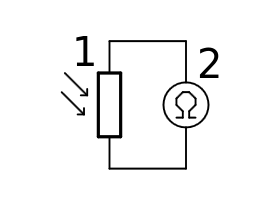
\includegraphics[ scale = 0.7]{Auf_1_2.PNG}
  	\caption[Schaltskizze zur Messung des Photowiderstandes]{Schaltskizze zur Messung des Photowiderstandes\footnotemark}
  \label{fig:auf_1_2}
\end{figure}
\footnotetext{Abbildung entnommen von http://www.atlas.uni-wuppertal.de/$\sim$kind/ep6\_14.pdf Seite 2 am 01.12.2014}

\subsubsection*{Versuchsdurchführung}
%erklären, !was! wir machen, !warum! wir das machen und mit welchem ziel
%(wichtig) präzize erklären, wie bei dem versuch vorgegangen und was gemacht wurde

Der Photowiderstand wird in das DMM eingesteckt und der Widerstand bei starker Beleuchtung (Fenster, Lampe), mittlerer Beleuchtung und schwacher Beleuchtung (abgedeckt mit der Hand). Dann wird noch ein Lichtstärkefilter von 20\%-100\%, der in 20\% Schritten skaliert ist verwendet und für jede Einstellung der Widerstand gemessen.

\subsubsection*{Messergebnisse}
%die messwerte in !übersichtlichen! tabellen angegeben
%zu viele kleine tabellen in große tabellen überführen!
%zu große tabellen mit dem [scale]-befehl scalieren oder (falls zu lang) in zwei kleinere tabellen aufteilen
%(wichtig) vor !jeder! tabelle sagen, was gemessen wurde und wie die fehler gewählt wurden und ausreichend !erklären!, !warum! wir unsere fehler grade so gewählt haben

Der Fehler des Widerstandwertes wurde mit dem Ablesefehler und dem angegebenen Fehler bestimmt und beträgt bei allen Werten 6$\Omega$ außer bei dem 25500$\Omega$ Widerstandswert, da liegt er bei 60$\Omega$

\begin{table}[H]
\centering
\begin{tabular}{|r|r|r|}
\hline
\multicolumn{1}{|l|}{Filter/\%} & \multicolumn{1}{l|}{Widerstand/$\Omega$} \\ \hline
100 & 435 \\ \hline
80 & 570 \\ \hline
60 & 600 \\ \hline
40 & 830 \\ \hline
20 & 1300 \\ \hline
0 & 25500 \\ \hline
\end{tabular}
\caption{Messdaten des Widerstandes in Abhängigkeit der Lichtstärke}
\label{tab:1_2}
\end{table}


\subsubsection*{Auswertung}
%zuerst !alle! errechneten werte entweder in ganzen sätzen aufzählen, oder in tabellen (übersichtlicher) dargestellen, sowie auf die verwendeten formeln verweisen (die referenzierung der formel kann in der überschrift stehen)
%kurz erwähnen (vor der tabelle), warum wir das ganze ausrechnen bzw. was wir dort ausrechnen
%danach histogramme und plots erstellen, wobei wenn möglich funktionen durch die plots gelegt werden (zur not können auch splines benutzt werden, was aber angegeben werden muss)
%bei fits immer die funktion und das reduzierte chiquadrat mit angegeben, wobei auf verständlichkeit beim entziffern der zehnerpotenzen geachtet werden muss z.b. f(x)=(wert+-fehler)\cdot10^{irgendeine zahl}\cdot x + (wert+-fehler)\cdot10^{irgendeine zahl}
%bei jedem fit erklären, nach welchem zusammenhang gefittet wurde und warum!
%bei plots darauf achten, dass die achsenbeschriftung (auch die tics) die richtige größe haben und die legende im plot nicht die messwerte verdeckt
%kurz die aufgabenstellung abhandeln
%2-----------------------------------------------2

Plottet man die gemessenen Werte aus Tabelle \ref{tab:1_2} so ergibt sich der Plot in Abbildung \ref{fig:1_2}.

\begin{figure}[H] 
  \centering
    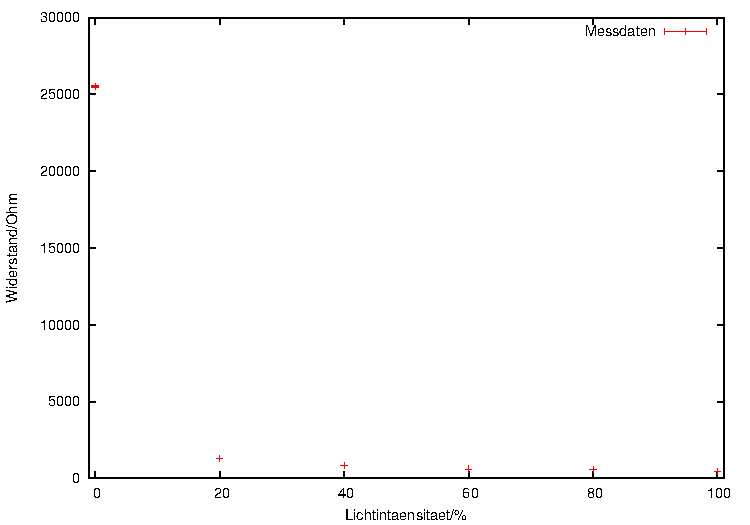
\includegraphics[ scale = 1]{1_2.pdf}
  	\caption[Daten aus der Messung des Widerstandes in Abhängigkeit der Lichtintensität]{Daten aus der Messung des Widerstandes in Abhängigkeit der Lichtintensität}
  \label{fig:1_2}
\end{figure}

\subsubsection*{Diskussion}
%(immer) die gemessenen werte und die bestimmten werte über die messfehler mit literaturwerten oder untereinander vergleichen
%in welchem fehlerintervall des messwertes liegt der literaturwert oder der vergleichswert?
%wie ist der relative anteil des fehlers am messwert und damit die qualität unserer messung?
%in einem satz erklären, wie gut unser fehler und damit unsere messung ist
%kurz erläutern, wie systematische fehler unsere messung beeinflusst haben könnten
%(wichtig) zum schluss ansprechen, in wie weit die ergebnisse mit der theoretischen vorhersage übereinstimmen
%--------------------------------------------------------------------------------------------
%falls tabellen mit den messwerten zu lang werden, kann die section mit den messwerten auch hinter der diskussion angefügt bzw. eine section mit dem anhang eingefügt werden.
%1-----------------------------------------------1

Wie erwartet stieg der Widerstand bei sinkender Intensität.

\subsection{Photodiode}
%kurz das ziel dieses versuchsteiles ansprechen, damit keine zwei überschriften direkt übereinander stehen!
%bei schwierigeren versuchen kann auch der theoretische hintergrund erläutert werden. (mit formeln, herleitungen und erklärungen)

In diesem Versuchsteil wird eine Photodiode zur Bestimmung der Lichtintensität verwendet. Die Abhängigkeit der Lichtintensität ist linear zum erzeugten Strom und die Änderung der Stromstärke erfolgt näherungsweise instantan. Jedoch ist der Photostrom sehr klein und die Messung ist stark von der Wellenlänge des Lichtes abhängig.

\subsubsection*{Verwendete Geräte}
%(immer) eine skizze oder ein foto einfügen, die geräte/materialien !nummerieren! und z.b. eine legende dazu schreiben, besser wäre es das ganze in einem Fließtext gut zu beschreiben.
%falls am anfang des versuches nicht klar ist, was alles verwendet wird, wenn möglich erst am ende ein großes foto von den verwendeten materialien machen!\\

Es werden eine Photodiode und ein DMM verwendet.


\subsubsection*{Versuchsaufbau}
%skizze zum versuchsaufbau (oder foto) einfügen,   es muss erklärt werden wie das ganze funktioniert und welche speziellen einstellungen verwendet wurden (z.b. welche knöpfe an den geräten für die messung verdreht wurden)

1 ist die Photodiode, 2 und 3 ist das DMM.

\begin{figure}[H] 
  \centering
    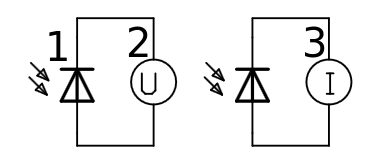
\includegraphics[ scale = 0.7]{Auf_1_3.PNG}
  	\caption[Schaltskizze zur Messung der Photodiode]{Schaltskizze zur Messung der Photodiode\footnotemark}
  \label{fig:auf_1_3}
\end{figure}
\footnotetext{Abbildung entnommen von http://www.atlas.uni-wuppertal.de/$\sim$kind/ep6\_14.pdf Seite 3 am 01.12.2014}

\subsubsection*{Versuchsdurchführung}
%erklären, !was! wir machen, !warum! wir das machen und mit welchem ziel
%(wichtig) präzize erklären, wie bei dem versuch vorgegangen und was gemacht wurde

Die Photodiode wird in das DMM eingesetzt, einmal so das der Photostrom und ein mal die Photospannung gemessen werden. Dann wird wieder der Lichtstärkefilter von 20\% bis 100\%, mit 20\% Schritten verwendet und jeweils der Photostrom und die Photospannung gemessen.

\subsubsection*{Messergebnisse}
%die messwerte in !übersichtlichen! tabellen angegeben
%zu viele kleine tabellen in große tabellen überführen!
%zu große tabellen mit dem [scale]-befehl scalieren oder (falls zu lang) in zwei kleinere tabellen aufteilen
%(wichtig) vor !jeder! tabelle sagen, was gemessen wurde und wie die fehler gewählt wurden und ausreichend !erklären!, !warum! wir unsere fehler grade so gewählt haben

Der Fehler wurde mit dem Ablesefehler und dem angegebenem Fehler bestimmt, er beträgt 0,006mA bzw. 0,006V.

\begin{table}[H]
\centering
\begin{tabular}{|r|r|r|}
\hline
\multicolumn{1}{|l|}{Filter/\%} & \multicolumn{1}{l|}{Strom/mA} & \multicolumn{1}{l|}{Spannung/V} \\ \hline
100 & 0,005 & 0,303 \\ \hline
80 & 0,004 & 0,297 \\ \hline
60 & 0,003 & 0,292 \\ \hline
40 & 0,002 & 0,274 \\ \hline
20 & 0,001 & 0,256 \\ \hline
0 & 0 & 0,136 \\ \hline
\end{tabular}
\caption{Messdaten des Stroms/der Spannung in Abhängigkeit der Lichtstärke}
\label{tab:1_3}
\end{table}



\subsubsection*{Auswertung}
%zuerst !alle! errechneten werte entweder in ganzen sätzen aufzählen, oder in tabellen (übersichtlicher) dargestellen, sowie auf die verwendeten formeln verweisen (die referenzierung der formel kann in der überschrift stehen)
%kurz erwähnen (vor der tabelle), warum wir das ganze ausrechnen bzw. was wir dort ausrechnen
%danach histogramme und plots erstellen, wobei wenn möglich funktionen durch die plots gelegt werden (zur not können auch splines benutzt werden, was aber angegeben werden muss)
%bei fits immer die funktion und das reduzierte chiquadrat mit angegeben, wobei auf verständlichkeit beim entziffern der zehnerpotenzen geachtet werden muss z.b. f(x)=(wert+-fehler)\cdot10^{irgendeine zahl}\cdot x + (wert+-fehler)\cdot10^{irgendeine zahl}
%bei jedem fit erklären, nach welchem zusammenhang gefittet wurde und warum!
%bei plots darauf achten, dass die achsenbeschriftung (auch die tics) die richtige größe haben und die legende im plot nicht die messwerte verdeckt
%kurz die aufgabenstellung abhandeln
%2-----------------------------------------------2

Plottet man die Werte aus Tabelle \ref{tab:1_3} für die Spannung, ergibt sich die Grafik in Abbildung \ref{fig:1_3_U}. Es ist deutlich der logarithmische Verlauf zu erkennen.


\begin{figure}[H] 
  \centering
    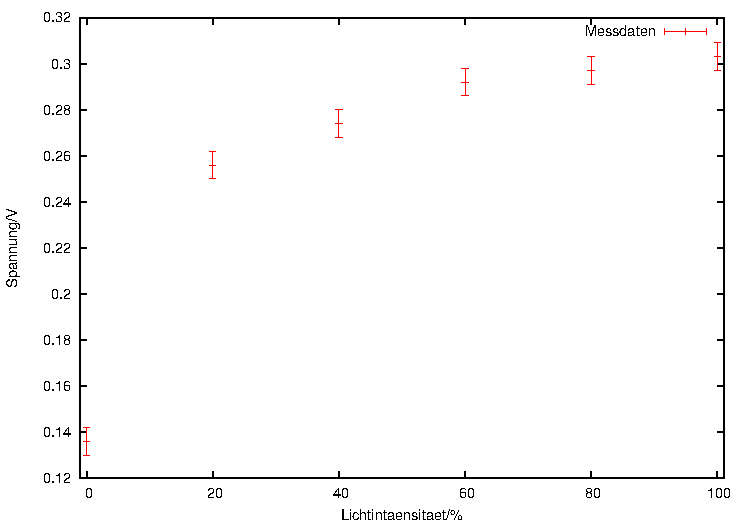
\includegraphics[ scale = 1]{1_3_U.pdf}
  	\caption[Daten aus der Messung der Spannung in Abhängigkeit der Lichtintensität]{Daten aus der Messung der Spannung in Abhängigkeit der Lichtintensität}
  \label{fig:1_3_U}
\end{figure}

Plottet man die Werte aus Tabelle \ref{tab:1_3} für den Strom, ergibt sich die Grafik in Abbildung \ref{fig:1_3_A}. Es lässt sich deutlich der lineare Verlauf erkennen.

\begin{figure}[H] 
  \centering
    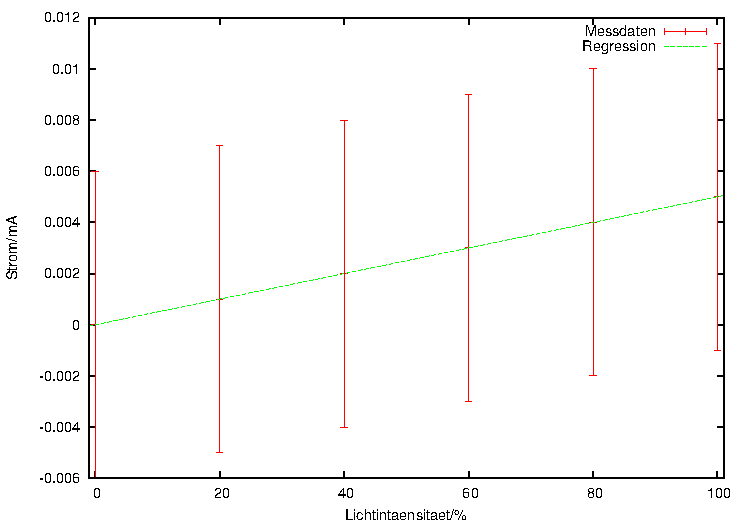
\includegraphics[ scale = 1]{1_3_A.pdf}
  	\caption[Daten aus der Messung des Stroms in Abhängigkeit der Lichtintensität]{Daten aus der Messung des Stroms in Abhängigkeit der Lichtintensität}
  \label{fig:1_3_A}
\end{figure}

\subsubsection*{Diskussion}
%(immer) die gemessenen werte und die bestimmten werte über die messfehler mit literaturwerten oder untereinander vergleichen
%in welchem fehlerintervall des messwertes liegt der literaturwert oder der vergleichswert?
%wie ist der relative anteil des fehlers am messwert und damit die qualität unserer messung?
%in einem satz erklären, wie gut unser fehler und damit unsere messung ist
%kurz erläutern, wie systematische fehler unsere messung beeinflusst haben könnten
%(wichtig) zum schluss ansprechen, in wie weit die ergebnisse mit der theoretischen vorhersage übereinstimmen
%--------------------------------------------------------------------------------------------
%falls tabellen mit den messwerten zu lang werden, kann die section mit den messwerten auch hinter der diskussion angefügt bzw. eine section mit dem anhang eingefügt werden.
%1-----------------------------------------------1

Wie erwartet ergab sich für die Spannungsmessung ein logarithmischer Verlauf und für die Strommessung ein linearer Verlauf.
Besser wäre es gewesen den Strom über dem Innenwiderstand des DVMs zu messen, da unsere Fehler nun größer als die Ströme selber sind.

\subsection{Phototransistor}
%kurz das ziel dieses versuchsteiles ansprechen, damit keine zwei überschriften direkt übereinander stehen!
%bei schwierigeren versuchen kann auch der theoretische hintergrund erläutert werden. (mit formeln, herleitungen und erklärungen)

In diesem Versuchsteil wird die Lichtstärke mittels eines Phototransistors gemessen. Der Phototransistor hat den Vorteil, dass die Photostrom um das bis zu 100-fache verstärkt wird.

\subsubsection*{Verwendete Geräte}
%(immer) eine skizze oder ein foto einfügen, die geräte/materialien !nummerieren! und z.b. eine legende dazu schreiben, besser wäre es das ganze in einem Fließtext gut zu beschreiben.
%falls am anfang des versuches nicht klar ist, was alles verwendet wird, wenn möglich erst am ende ein großes foto von den verwendeten materialien machen!\\

Es werden ein Widerstände, ein Phototransistor, ein DMM, eine Photodiode, ein Oszilloskop, ein Funktionsgenerator und eine Spannungsquelle verwendet.

\subsubsection*{Versuchsaufbau}
%skizze zum versuchsaufbau (oder foto) einfügen,   es muss erklärt werden wie das ganze funktioniert und welche speziellen einstellungen verwendet wurden (z.b. welche knöpfe an den geräten für die messung verdreht wurden)

U0 ist eine 10V Spannungsquelle, R1 ein 1k$\Omega$ Widerstand, I ein DMM und T1 der Phototransistor.

\begin{figure}[H] 
  \centering
    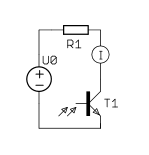
\includegraphics[ scale = 1]{Auf_1_4_1.PNG}
  	\caption[Schaltskizze zur Messung mit dem Phototransistor]{Schaltskizze zur Messung mit dem Phototransistor\footnotemark}
  \label{fig:auf_1_4_1}
\end{figure}
\footnotetext{Abbildung entnommen von http://www.atlas.uni-wuppertal.de/$\sim$kind/ep6\_14.pdf Seite 3 am 01.12.2014}

1 ist der Funktionsgenerator, 2 ein 1k$\Omega$ Widerstand, 3 eine Photodiode, 4 ein 100k$\Omega$ Widerstand und 5 der Phototransistor.

\begin{figure}[H] 
  \centering
    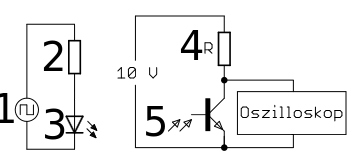
\includegraphics[ scale = 0.7]{Auf_1_4_2.PNG}
  	\caption[Schaltskizze zur Messung mit  Photodiode und Phototransistor]{Schaltskizze zur Messung mit  Photodiode und Phototransistor\footnotemark}
  \label{fig:auf_1_4_2}
\end{figure}
\footnotetext{Abbildung entnommen von http://www.atlas.uni-wuppertal.de/$\sim$kind/ep6\_14.pdf Seite 3 am 01.12.2014}



\subsubsection*{Versuchsdurchführung}
%erklären, !was! wir machen, !warum! wir das machen und mit welchem ziel
%(wichtig) präzize erklären, wie bei dem versuch vorgegangen und was gemacht wurde

In diesem Versuchsteil wird die Schaltung in Abbildung \ref{fig:auf_1_4_1} aufgebaut um den Strom durch den Transistor in Abhängigkeit der Lichtintensität zu messen. Zuerst wird das Raumlicht als Lichtquelle verwendet, im zweiten Teil \ref{fig:1_4_2} eine LED. Um die Lichtintensität zu regulieren wird ein Lichtstärkefilter von 20\% bis 100\%, mit 20\% Schritten verwendet. Im zweiten Teil wird die Schaltung aus Abbildung \ref{fig:auf_1_4_2} aufgebaut, der Phototransistor mit der Photodiode beleuchtet und die Kurve mit dem Oszilloskop aufgenommen. Die Diode ist dabei an ein Rechtecksignal angeschlossen, welches mit dem Phototransistor über das Oszilloskop aufgenommen wird.

\subsubsection*{Messergebnisse}
%die messwerte in !übersichtlichen! tabellen angegeben
%zu viele kleine tabellen in große tabellen überführen!
%zu große tabellen mit dem [scale]-befehl scalieren oder (falls zu lang) in zwei kleinere tabellen aufteilen
%(wichtig) vor !jeder! tabelle sagen, was gemessen wurde und wie die fehler gewählt wurden und ausreichend !erklären!, !warum! wir unsere fehler grade so gewählt haben

Der Fehler des Stroms wurde mit dem Ablesefehler und dem angegebenem Fehler bestimmt und beträgt 0,006mA.

\begin{table}[H]
\begin{center}
\begin{tabular}{|r|r|}
\hline
\multicolumn{1}{|l|}{Filter/\%} & \multicolumn{1}{l|}{Strom/mA} \\ \hline
100 & 0,058 \\ \hline
80 & 0,047 \\ \hline
60 & 0,037 \\ \hline
40 & 0,025 \\ \hline
20 & 0,014 \\ \hline
0 & 0,002 \\ \hline
\end{tabular}
\end{center}
\caption{Messdaten des Stroms in Abhängigkeit der Lichtstärke für den Phototransistor}
\label{tab:1_4_transistor}
\end{table}



Der Fehler des Stroms wurde mit dem Ablesefehler und dem angegebenem Fehler bestimmt und beträgt 0,06mA.

\begin{table}[H]
\begin{center}
\begin{tabular}{|r|r|}
\hline
\multicolumn{1}{|l|}{Filter/\%} & \multicolumn{1}{l|}{Strom/mA} \\ \hline
100 & 9,15 \\ \hline
80 & 9,15 \\ \hline
60 & 9,14 \\ \hline
40 & 9,14 \\ \hline
20 & 9,14 \\ \hline
0 & 9,14 \\ \hline
\end{tabular}
\end{center}
\caption{Messdaten des Stroms in Abhängigkeit der Lichtstärke für die Photodiode}
\label{tab:1_4_diode}
\end{table}


\subsubsection*{Auswertung}
%zuerst !alle! errechneten werte entweder in ganzen sätzen aufzählen, oder in tabellen (übersichtlicher) dargestellen, sowie auf die verwendeten formeln verweisen (die referenzierung der formel kann in der überschrift stehen)
%kurz erwähnen (vor der tabelle), warum wir das ganze ausrechnen bzw. was wir dort ausrechnen
%danach histogramme und plots erstellen, wobei wenn möglich funktionen durch die plots gelegt werden (zur not können auch splines benutzt werden, was aber angegeben werden muss)
%bei fits immer die funktion und das reduzierte chiquadrat mit angegeben, wobei auf verständlichkeit beim entziffern der zehnerpotenzen geachtet werden muss z.b. f(x)=(wert+-fehler)\cdot10^{irgendeine zahl}\cdot x + (wert+-fehler)\cdot10^{irgendeine zahl}
%bei jedem fit erklären, nach welchem zusammenhang gefittet wurde und warum!
%bei plots darauf achten, dass die achsenbeschriftung (auch die tics) die richtige größe haben und die legende im plot nicht die messwerte verdeckt
%kurz die aufgabenstellung abhandeln
%2-----------------------------------------------2

Plottet man die Daten aus Tabelle \ref{tab:1_4_transistor} so ergibt sich die Grafik in Abbildung \ref{fig:1_4_T}. Der lineare Verlauf ist gut zu sehen.

\begin{figure}[H] 
  \centering
    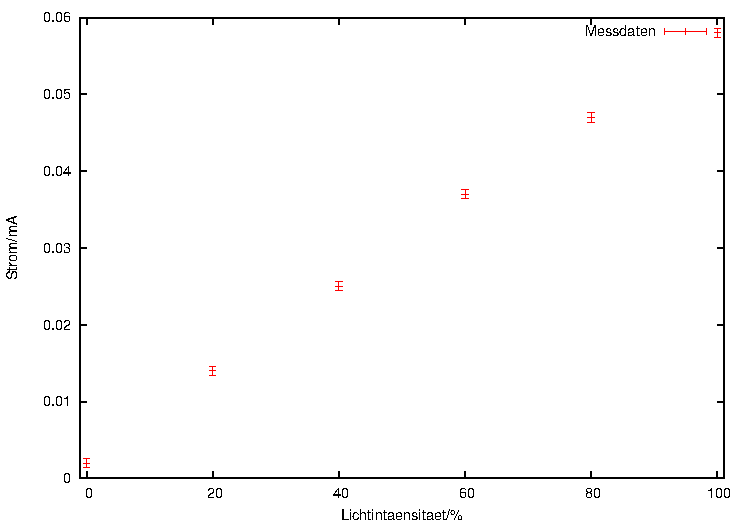
\includegraphics[ scale = 1]{1_4_T.pdf}
  	\caption[Daten aus der Messung des Stroms in Abhängigkeit der Lichtintensität für den Phototransistor]{Daten aus der Messung des Stroms in Abhängigkeit der Lichtintensität für den Phototransistor}
  \label{fig:1_4_T}
\end{figure}


Plottet man die Daten aus Tabelle \ref{tab:1_4_diode} so ergibt sich die Grafik in Abbildung \ref{fig:1_4_D}. Da des Auflösungsvermögen der Messapertur zu gering ist lässt sich kein linearer Verlauf erkennen. (Eine Möglichkeit wäre wie im letzten Versuchsteil die Messung des Stromes über den Innenwiderstand des DVMs für eine bessere Auflösung.)

\begin{figure}[H] 
  \centering
    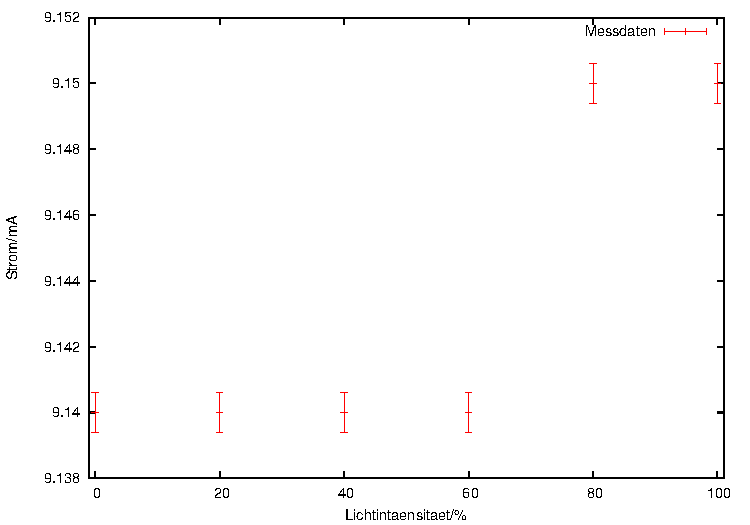
\includegraphics[ scale = 1]{1_4_D.pdf}
  	\caption[Daten aus der Messung des Stroms in Abhängigkeit der Lichtintensität für die Photodiode]{Daten aus der Messung des Stroms in Abhängigkeit der Lichtintensität für die Photodiode}
  \label{fig:1_4_D}
\end{figure}

Legt man das Signal des Phototransistors auf das Oszilloskop, welches von der Photodiode ausgesendet wird, so ergibt sich der Verlauf in Abbildung \ref{fig:auf_1_4_2}. Die Pulssignale sind deutlich in der Abbildung zu sehen.

\begin{figure}[H] 
  \centering
    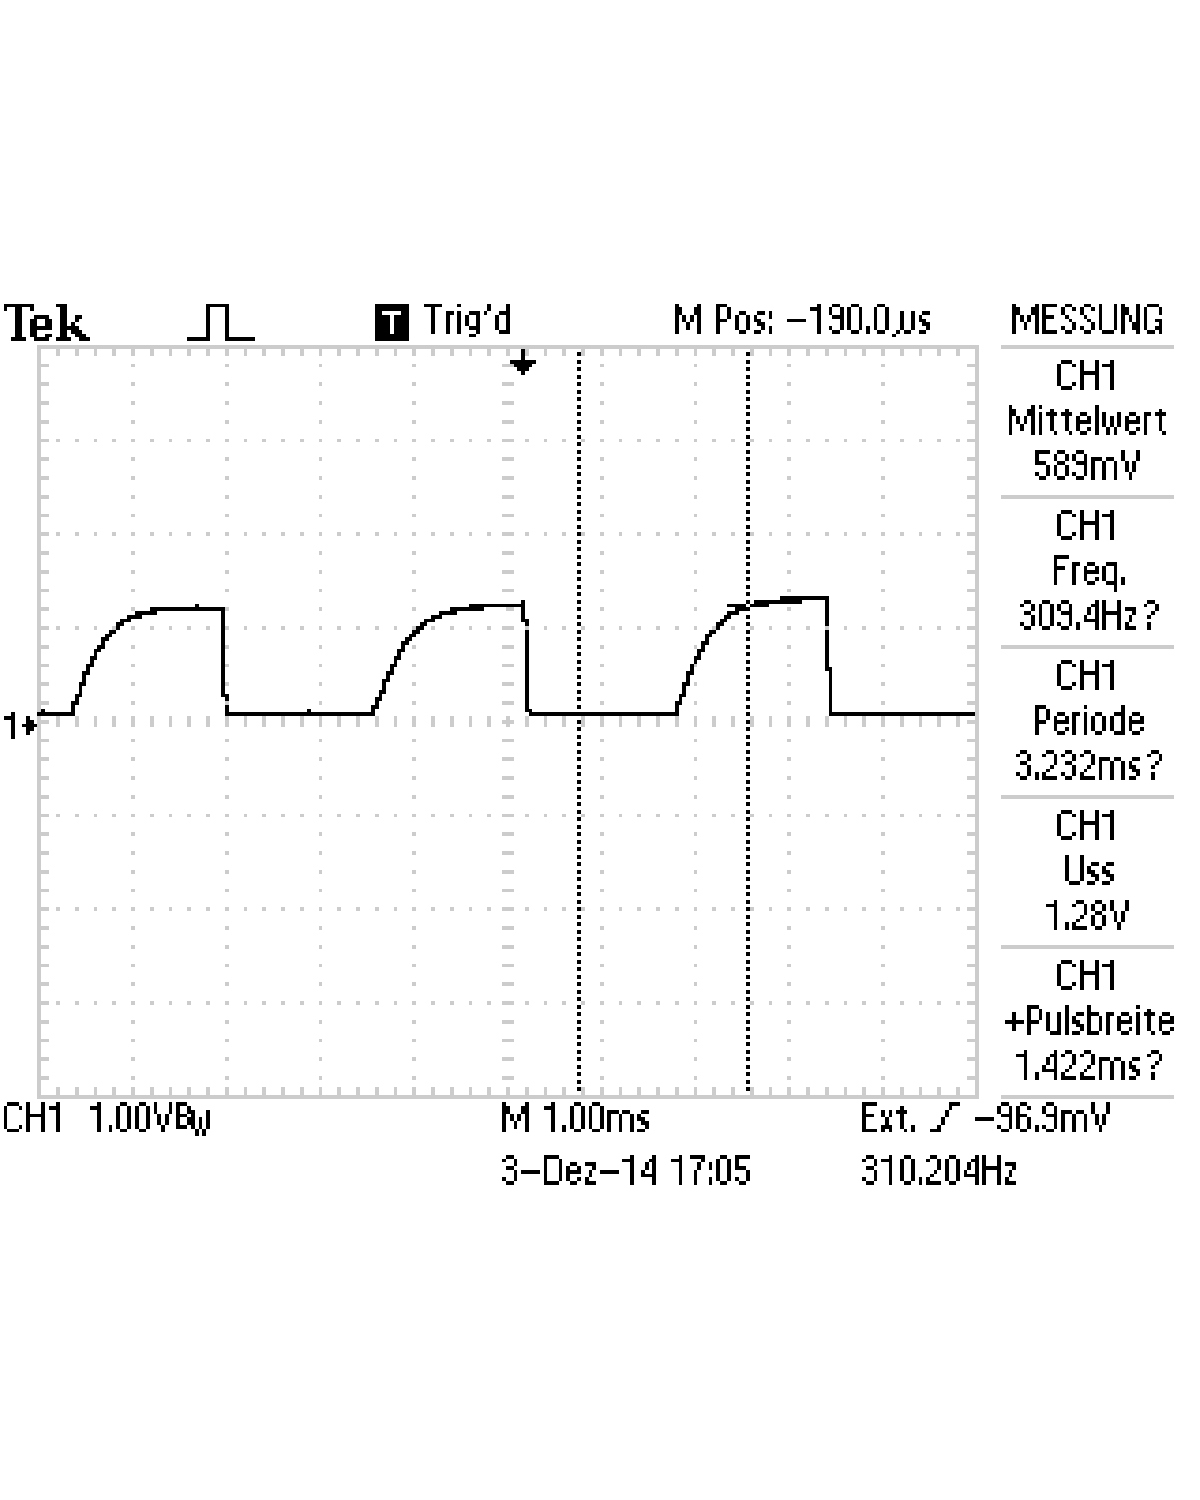
\includegraphics[ scale = 0.7]{1_4_2.pdf}
  	\caption[Aufnahme des Signals mit dem Oszilloskop]{Aufnahme des Signals mit dem Oszilloskop}
  \label{fig:1_4_2}
\end{figure}


\subsubsection*{Diskussion}
%(immer) die gemessenen werte und die bestimmten werte über die messfehler mit literaturwerten oder untereinander vergleichen
%in welchem fehlerintervall des messwertes liegt der literaturwert oder der vergleichswert?
%wie ist der relative anteil des fehlers am messwert und damit die qualität unserer messung?
%in einem satz erklären, wie gut unser fehler und damit unsere messung ist
%kurz erläutern, wie systematische fehler unsere messung beeinflusst haben könnten
%(wichtig) zum schluss ansprechen, in wie weit die ergebnisse mit der theoretischen vorhersage übereinstimmen
%--------------------------------------------------------------------------------------------
%falls tabellen mit den messwerten zu lang werden, kann die section mit den messwerten auch hinter der diskussion angefügt bzw. eine section mit dem anhang eingefügt werden.
%1-----------------------------------------------1

Wie erwartet ergibt sich ein linearer Zusammenhang zwischen der Lichtintensität und dem Strom. Der Zusammenhang ist bei bei der Messung mit der Photodiode nicht gut zu sehen, da die Auflösung des Messgerätes zu gering ist. Für diese Messung wäre es besser gewesen den Strom über den Innenwiderstand des DVMs zu messen. Der zeitlich unmittelbare Zusammenhang zwischen der Spannung und Lichteinstrahlung ist in Abbildung \ref{fig:1_4_2} zu sehen.


\subsection{Leuchtdiode als Lichtquelle}
%kurz das ziel dieses versuchsteiles ansprechen, damit keine zwei überschriften direkt übereinander stehen!
%bei schwierigeren versuchen kann auch der theoretische hintergrund erläutert werden. (mit formeln, herleitungen und erklärungen)

In diesem Versuchsteil wird die Leuchtdiode als Lichtquelle untersucht. Dazu wird bei verschiedenen Dioden die darüber abfallende Spannung gemessen.

\subsubsection*{Verwendete Geräte}
%(immer) eine skizze oder ein foto einfügen, die geräte/materialien !nummerieren! und z.b. eine legende dazu schreiben, besser wäre es das ganze in einem Fließtext gut zu beschreiben.
%falls am anfang des versuches nicht klar ist, was alles verwendet wird, wenn möglich erst am ende ein großes foto von den verwendeten materialien machen!\\

Es werden verschiedenfarbige Leuchtdioden, ein Netzgerät, Widerstände, eine Photodiode, ein Phototransistor, ein Oszilloskop, ein Potentiometer und ein Fingerpulsaufnehmer verwendet.

\subsubsection*{Versuchsaufbau}
%skizze zum versuchsaufbau (oder foto) einfügen,   es muss erklärt werden wie das ganze funktioniert und welche speziellen einstellungen verwendet wurden (z.b. welche knöpfe an den geräten für die messung verdreht wurden)

R ist ein 1k$\Omega$ Widerstand, 1 ist die Leuchtdiode und U ein DMM.

\begin{figure}[H] 
  \centering
    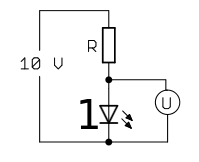
\includegraphics[ scale = 0.7]{Auf_1_5_1.PNG}
  	\caption[Schaltskizze zur Messung mit  Photodiode und Phototransistor]{Schaltskizze zur Messung mit  Photodiode und Phototransistor\footnotemark}
  \label{fig:auf_1_5_1}
\end{figure}
\footnotetext{Abbildung entnommen von http://www.atlas.uni-wuppertal.de/$\sim$kind/ep6\_14.pdf Seite 4 am 01.12.2014}

1 ist die Photodiode, 2 der Phototransistor, R\_LED ist ein 470$\Omega$ Widerstand und R\_Ph-Tr ist ein 10 bis 100k$\Omega$ Widerstand.

\begin{figure}[H] 
  \centering
    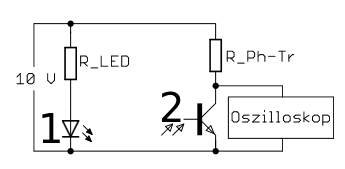
\includegraphics[ scale = 0.7]{Auf_1_5_2.PNG}
  	\caption[Schaltskizze zur Messung mit  Photodiode und Phototransistor]{Schaltskizze zur Messung mit  Photodiode und Phototransistor\footnotemark}
  \label{fig:auf_1_5_2}
\end{figure}
\footnotetext{Abbildung entnommen von http://www.atlas.uni-wuppertal.de/$\sim$kind/ep6\_14.pdf Seite 4 am 01.12.2014}

1 ist die Photodiode und 2 der Phototransistor.

\begin{figure}[H] 
  \centering
    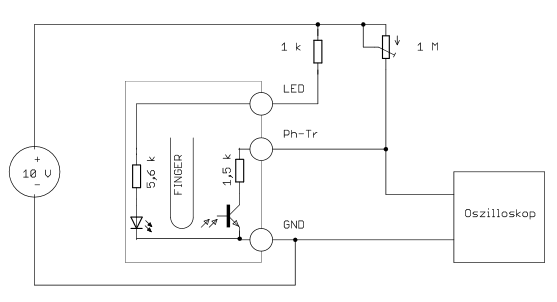
\includegraphics[ scale = 0.7]{Auf_1_5_3.PNG}
  	\caption[Schaltskizze zur Messung des Pulses]{Schaltskizze zur Messung des Pulses\footnotemark}
  \label{fig:auf_1_5_3}
\end{figure}
\footnotetext{Abbildung entnommen von http://www.atlas.uni-wuppertal.de/$\sim$kind/ep6\_14.pdf Seite 5 am 01.12.2014}


\subsubsection*{Versuchsdurchführung}
%erklären, !was! wir machen, !warum! wir das machen und mit welchem ziel
%(wichtig) präzize erklären, wie bei dem versuch vorgegangen und was gemacht wurde

Es wird die Schaltung aus Abbildung \ref{fig:auf_1_5_1} aufgebaut, verschiedene Dioden eingesetzt und jeweils die Spannung gemessen. Im zweitem Teil wird die Schaltung aus Abbildung \ref{fig:auf_1_5_2} aufgebaut. Mit der Leuchtdiode wird ein Signal an den Phototransistor geschickt dieses wird mit dem 0\% Intensitätsfilter  geblockt. Die resultierend Kurve wird mit dem Oszilloskop aufgenommen. Im letztem Teil wird die Schaltung aus Abbildung \ref{fig:auf_1_5_3} aufgebaut und der Puls mit dem Fingerpulsaufnehmer aufgenommen auf auf dem Oszilloskop ausgegeben.

\subsubsection*{Messergebnisse}
%die messwerte in !übersichtlichen! tabellen angegeben
%zu viele kleine tabellen in große tabellen überführen!
%zu große tabellen mit dem [scale]-befehl scalieren oder (falls zu lang) in zwei kleinere tabellen aufteilen
%(wichtig) vor !jeder! tabelle sagen, was gemessen wurde und wie die fehler gewählt wurden und ausreichend !erklären!, !warum! wir unsere fehler grade so gewählt haben

Der Fehler der Spannung wurde mit dem Ablesefehler bestimmt und beträgt 0,1V.

\begin{table}[H]
\begin{center}
\begin{tabular}{|l|r|}
\hline
Farbe & \multicolumn{1}{l|}{Spannung/V} \\ \hline
Rot & 1,79 \\ \hline
Gelb & 1,89 \\ \hline
Blau & 3,69 \\ \hline
Dunkel & 1,09 \\ \hline
Grün & 1,97 \\ \hline
Weis & 3,13 \\ \hline
\end{tabular}
\end{center}
\caption{Spannungen die über den Dioden abfallen}
\label{tab:1_5}
\end{table}


\subsubsection*{Auswertung}
%zuerst !alle! errechneten werte entweder in ganzen sätzen aufzählen, oder in tabellen (übersichtlicher) dargestellen, sowie auf die verwendeten formeln verweisen (die referenzierung der formel kann in der überschrift stehen)
%kurz erwähnen (vor der tabelle), warum wir das ganze ausrechnen bzw. was wir dort ausrechnen
%danach histogramme und plots erstellen, wobei wenn möglich funktionen durch die plots gelegt werden (zur not können auch splines benutzt werden, was aber angegeben werden muss)
%bei fits immer die funktion und das reduzierte chiquadrat mit angegeben, wobei auf verständlichkeit beim entziffern der zehnerpotenzen geachtet werden muss z.b. f(x)=(wert+-fehler)\cdot10^{irgendeine zahl}\cdot x + (wert+-fehler)\cdot10^{irgendeine zahl}
%bei jedem fit erklären, nach welchem zusammenhang gefittet wurde und warum!
%bei plots darauf achten, dass die achsenbeschriftung (auch die tics) die richtige größe haben und die legende im plot nicht die messwerte verdeckt
%kurz die aufgabenstellung abhandeln
%2-----------------------------------------------2

Die Spannung, die über den Dioden abfällt in Abhängigkeit der Farbe finden sich in Tabelle \ref{tab:1_5}.
\\ 
\\
Legt man das Signal des Phototransistors auf das Oszilloskop und stört die Signal Übertragung so ergibt sich der Verlauf in Abbildung \ref{fig:1_5_2}. Es ist deutlich zu sehen, das die Spannung ansteigt, sobald die Übertragung unterbrochen wird.

\begin{figure}[H] 
  \centering
    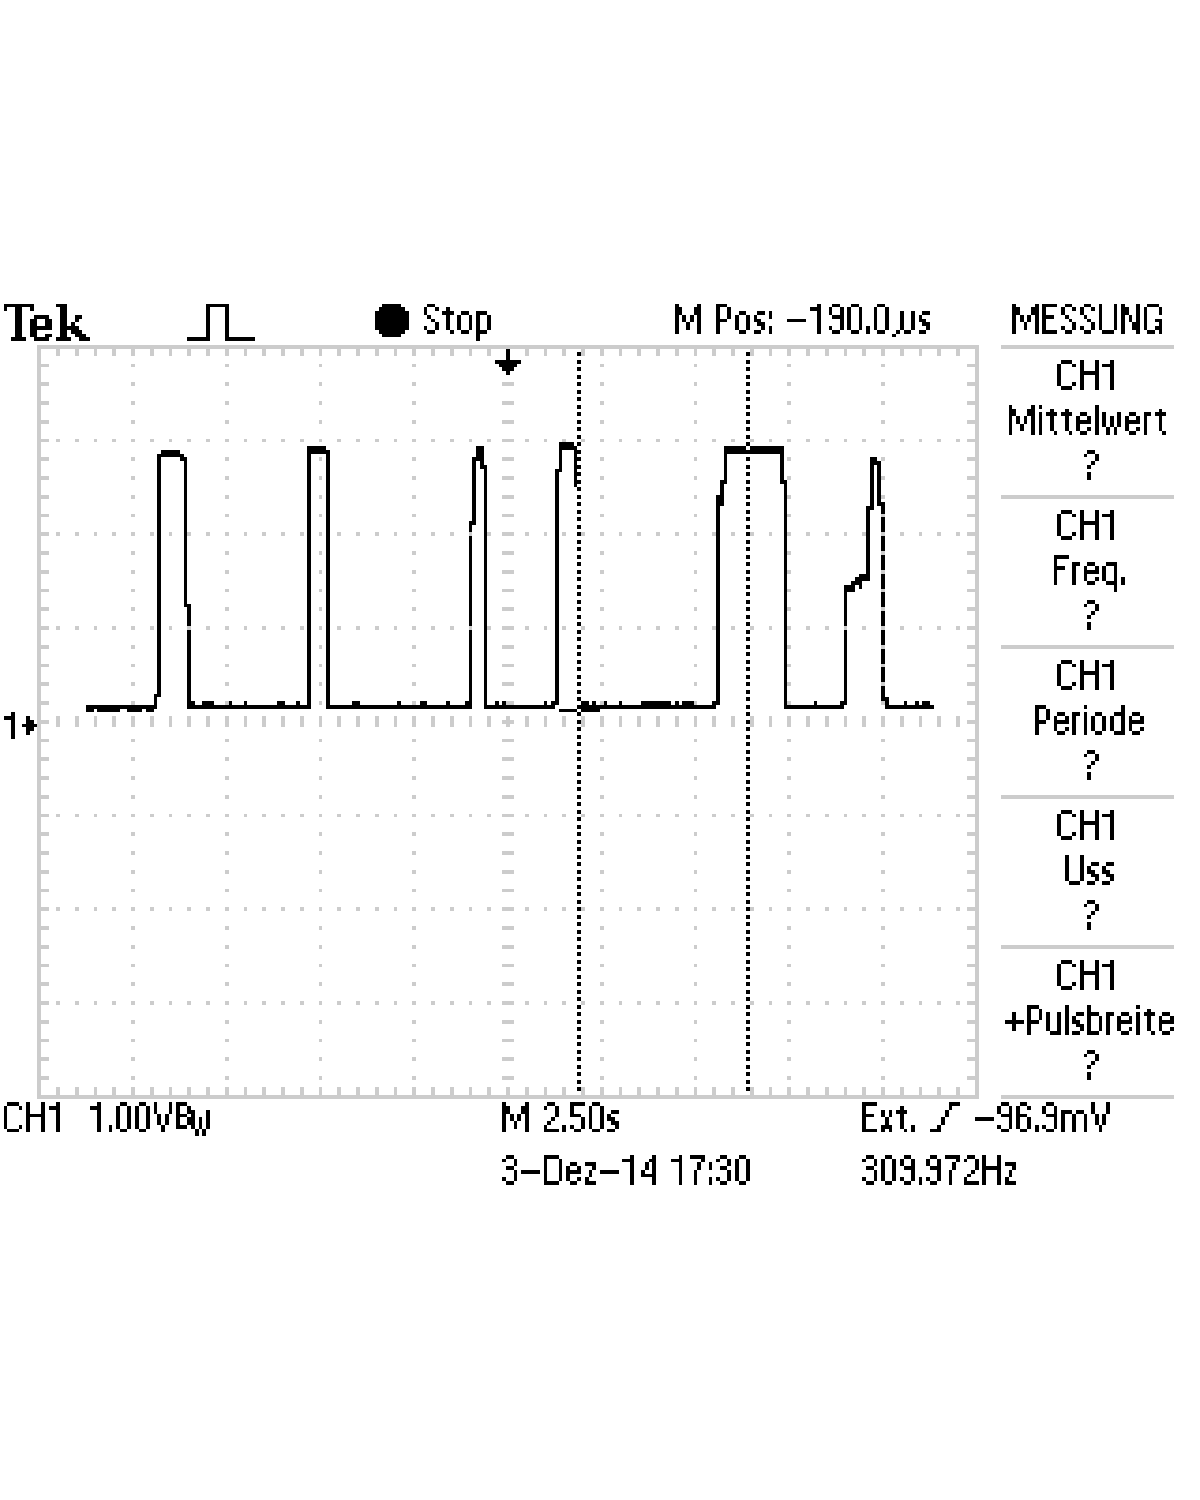
\includegraphics[ scale = 0.7]{1_5_2.pdf}
  	\caption[Aufnahme des Signals mit dem Oszilloskop]{Aufnahme des Signals mit dem Oszilloskop}
  \label{fig:1_5_2}
\end{figure}

Bei der Messung des Pulses ergab sich der Verlauf in Abbildung \ref{fig:auf_1_5_3}. Es ist deutlich der Puls der Person zu sehen.

\begin{figure}[H] 
  \centering
    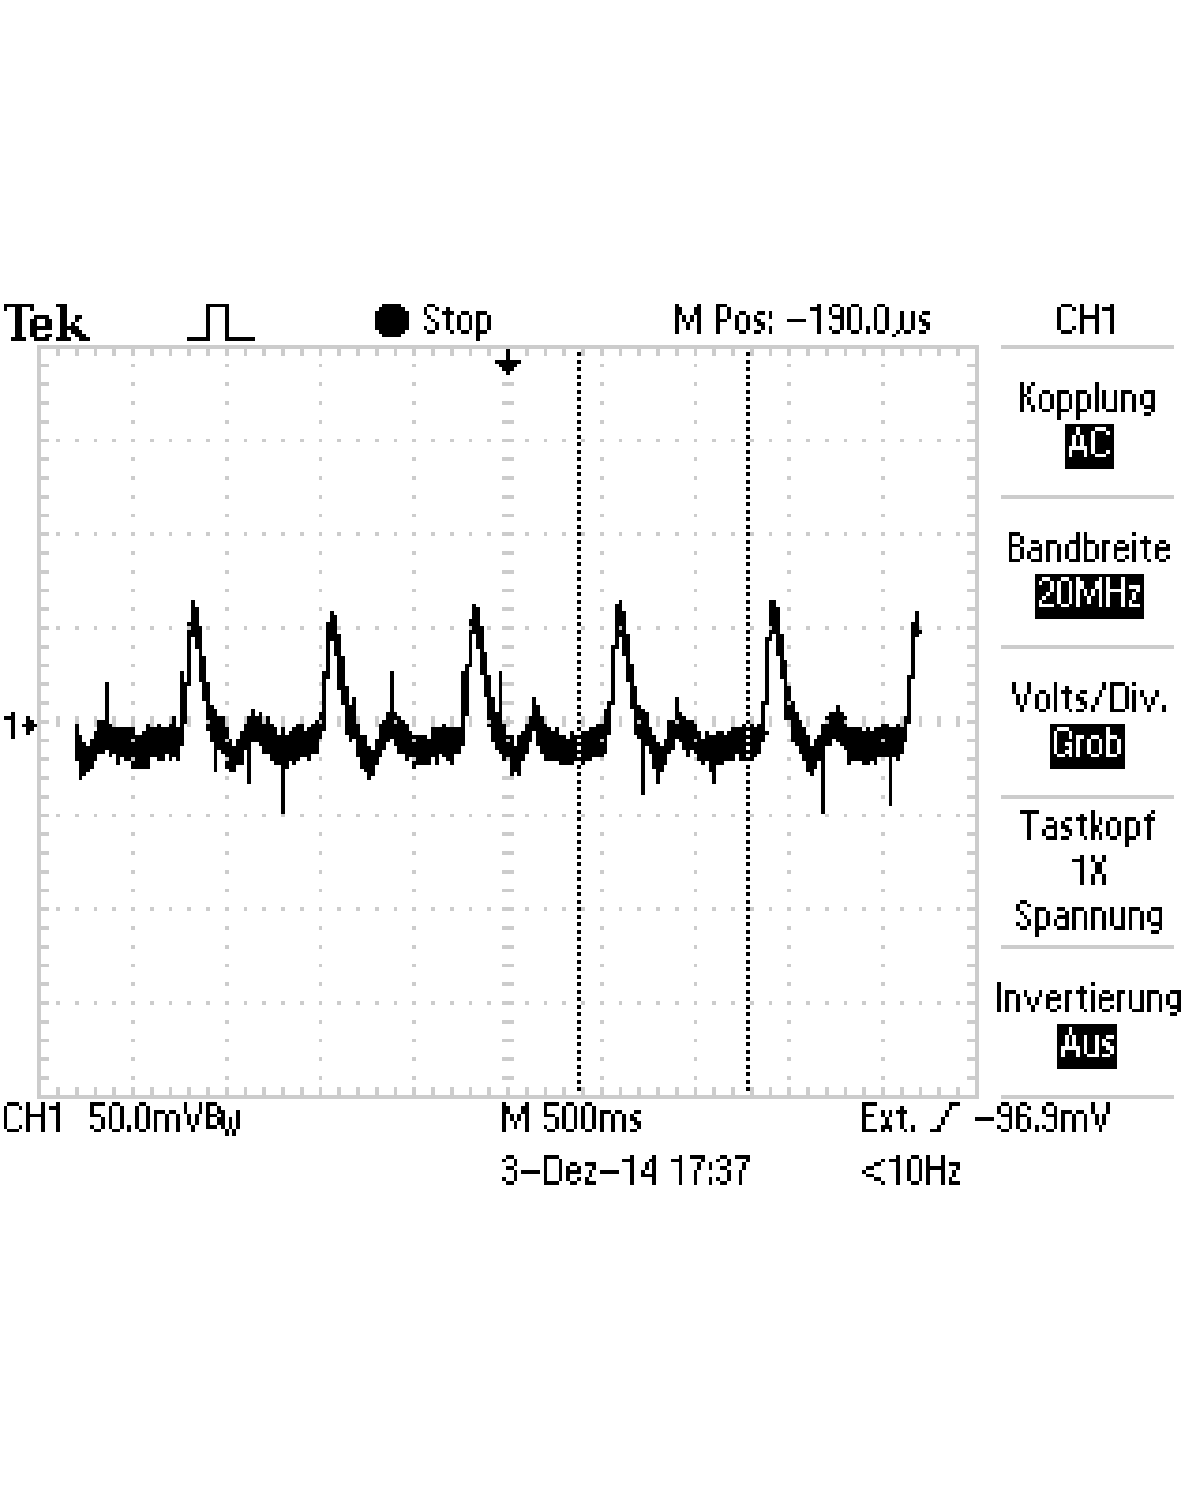
\includegraphics[ scale = 0.7]{1_5_3.pdf}
  	\caption[Aufnahme des Signals mit dem Oszilloskop]{Aufnahme des Signals mit dem Oszilloskop}
  \label{fig:1_5_3}
\end{figure}

\subsubsection*{Diskussion}
%(immer) die gemessenen werte und die bestimmten werte über die messfehler mit literaturwerten oder untereinander vergleichen
%in welchem fehlerintervall des messwertes liegt der literaturwert oder der vergleichswert?
%wie ist der relative anteil des fehlers am messwert und damit die qualität unserer messung?
%in einem satz erklären, wie gut unser fehler und damit unsere messung ist
%kurz erläutern, wie systematische fehler unsere messung beeinflusst haben könnten
%(wichtig) zum schluss ansprechen, in wie weit die ergebnisse mit der theoretischen vorhersage übereinstimmen
%--------------------------------------------------------------------------------------------
%falls tabellen mit den messwerten zu lang werden, kann die section mit den messwerten auch hinter der diskussion angefügt bzw. eine section mit dem anhang eingefügt werden.
%1-----------------------------------------------1

Die Spannung der Photodioden entsprechen den erwarteten Werten. Im Teil danach ist wie erwartet zu erkenne, dass wenn das Signal unterbrochen wird die Spannung ansteigt, was so erwartet wurde. Der Puls konnte deutlich gemessen werden.



\section{Temperaturmessung}

In diesem Versuchsteil soll mit PTCs, NTCs und einem Thermoelement eine Temperaturmessung durchgeführt werden und im Anschluss die Eignung der verschiedenen Sensoren besprochen werden.


\subsection{PTCs}
%kurz das ziel dieses versuchsteiles ansprechen, damit keine zwei überschriften direkt übereinander stehen!
%bei schwierigeren versuchen kann auch der theoretische hintergrund erläutert werden. (mit formeln, herleitungen und erklärungen)

Der PTC ist ein Material, welches einen Temperaturabhängigen Widerstand hat, welcher bei Temperaturerhöhung ansteigt. Es wird sehr häufig Platin verwendet, da Platin einen sehr linearen Widerstandsanstieg in Abhängigkeit der Temperatur hat.

\subsubsection*{Verwendete Geräte}
%(immer) eine skizze oder ein foto einfügen, die geräte/materialien !nummerieren! und z.b. eine legende dazu schreiben, besser wäre es das ganze in einem Fließtext gut zu beschreiben.
%falls am anfang des versuches nicht klar ist, was alles verwendet wird, wenn möglich erst am ende ein großes foto von den verwendeten materialien machen!\\

Verwendet werden ein Pt1000 Sensor und ein DMM.

\subsubsection*{Verwendete Formeln}
%eine legende kann angefertigt werden, die selbstverständlichen buchstaben müssen nicht extra erklärt werden
%mit knappen erklärungen die !verwendeten! formeln, sowie die zugehörige fehlerrechnung einfügen
%2-----------------------------------------------2
%ab hier kann nochmal in einzelne versuchsteile unterteilt werden

Der Zusammenhang zwischen der Temperatur und dem Widerstand ist durch Gleichung \ref{eqn:ptc} gegeben.

\begin{align}
\text{R}(\text{T}) = \text{R}_0(1+\alpha \text{T})
\label{eqn:ptc}
\end{align}

\subsubsection*{Versuchsaufbau}
%skizze zum versuchsaufbau (oder foto) einfügen,   es muss erklärt werden wie das ganze funktioniert und welche speziellen einstellungen verwendet wurden (z.b. welche knöpfe an den geräten für die messung verdreht wurden)

1 ist der Pt1000 und 2 das DMM.

\begin{figure}[H] 
  \centering
    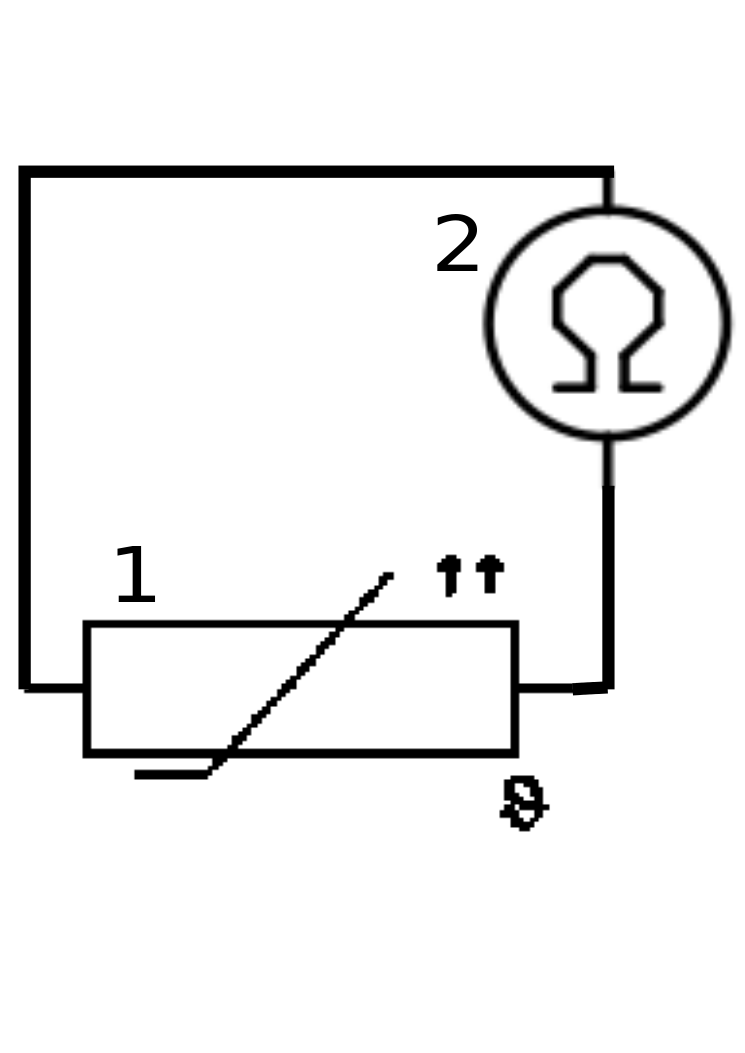
\includegraphics[ scale = 0.1]{Auf_2_1.png}
  	\caption[Schaltskizze zur Messung der Temperatur mit einem PTC]{Schaltskizze zur Messung der Temperatur mit einem PTC\footnotemark}
  \label{fig:auf_2_1}
\end{figure}
\footnotetext{Abbildungsteile entnommen von http://www.atlas.uni-wuppertal.de/$\sim$kind/ep6\_14.pdf am 01.12.2014}

\subsubsection*{Versuchsdurchführung}
%erklären, !was! wir machen, !warum! wir das machen und mit welchem ziel
%(wichtig) präzize erklären, wie bei dem versuch vorgegangen und was gemacht wurde

Der PTC wird an das DMM angeschlossen und der Widerstand bei Raumtemperatur und bei Handtemperatur gemessen.

\subsubsection*{Messergebnisse}
%die messwerte in !übersichtlichen! tabellen angegeben
%zu viele kleine tabellen in große tabellen überführen!
%zu große tabellen mit dem [scale]-befehl scalieren oder (falls zu lang) in zwei kleinere tabellen aufteilen
%(wichtig) vor !jeder! tabelle sagen, was gemessen wurde und wie die fehler gewählt wurden und ausreichend !erklären!, !warum! wir unsere fehler grade so gewählt haben

Die Fehler des Widerstandes wurde mit dem angegebenen Fehler und der Ableseungenauigkeit bestimmt und beträgt 6$\Omega$. Der Fehler der Temperatur wurde über die Ableseungenauigkeit bestimmt und beträgt 0,1C.

\begin{table}[H]
\begin{center}
\begin{tabular}{|r|r|}
\hline
\multicolumn{1}{|l|}{Temperatur/C} & \multicolumn{1}{l|}{Widerstand/$\Omega$} \\ \hline
24,4 & 1102 \\ \hline
35,5 & 1135 \\ \hline
\end{tabular}
\end{center}
\caption{Widerstand in Abhängigkeit der Temperatur}
\label{tab:2_1}
\end{table}


\subsubsection*{Auswertung}
%zuerst !alle! errechneten werte entweder in ganzen sätzen aufzählen, oder in tabellen (übersichtlicher) dargestellen, sowie auf die verwendeten formeln verweisen (die referenzierung der formel kann in der überschrift stehen)
%kurz erwähnen (vor der tabelle), warum wir das ganze ausrechnen bzw. was wir dort ausrechnen
%danach histogramme und plots erstellen, wobei wenn möglich funktionen durch die plots gelegt werden (zur not können auch splines benutzt werden, was aber angegeben werden muss)
%bei fits immer die funktion und das reduzierte chiquadrat mit angegeben, wobei auf verständlichkeit beim entziffern der zehnerpotenzen geachtet werden muss z.b. f(x)=(wert+-fehler)\cdot10^{irgendeine zahl}\cdot x + (wert+-fehler)\cdot10^{irgendeine zahl}
%bei jedem fit erklären, nach welchem zusammenhang gefittet wurde und warum!
%bei plots darauf achten, dass die achsenbeschriftung (auch die tics) die richtige größe haben und die legende im plot nicht die messwerte verdeckt
%kurz die aufgabenstellung abhandeln
%2-----------------------------------------------2

Fittet man die Messdaten auf Tabelle \ref{tab:2_1} nach Gleichung \ref{eqn:ptc} so ergibt sich $\alpha$ mit 0,0039$\pm$0,0002, das reduzierte Chi-Quadrat ergibt sich mit 2,45. 

\begin{figure}[H] 
  \centering
    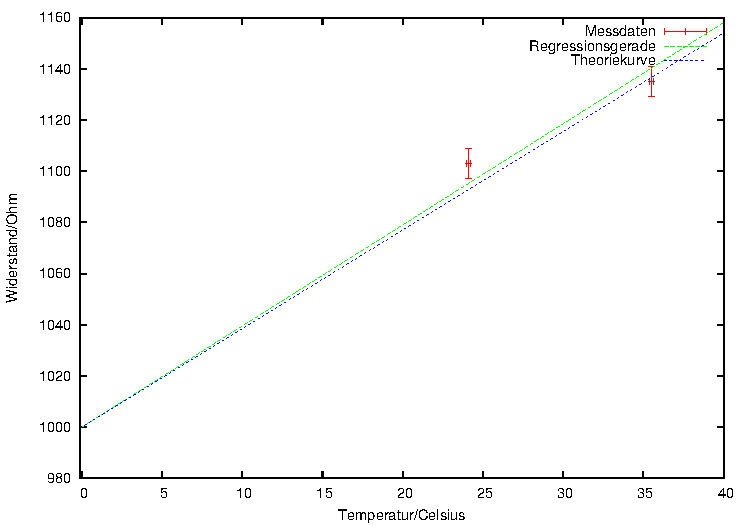
\includegraphics[ scale = 0.7]{2_1.pdf}
  	\caption[Daten der Messung, des Widerstandes in Abhängigkeit der Temperatur]{Daten der Messung, des Widerstandes in Abhängigkeit der Temperatur}
  \label{fig:2_1}
\end{figure}


\subsubsection*{Diskussion}
%(immer) die gemessenen werte und die bestimmten werte über die messfehler mit literaturwerten oder untereinander vergleichen
%in welchem fehlerintervall des messwertes liegt der literaturwert oder der vergleichswert?
%wie ist der relative anteil des fehlers am messwert und damit die qualität unserer messung?
%in einem satz erklären, wie gut unser fehler und damit unsere messung ist
%kurz erläutern, wie systematische fehler unsere messung beeinflusst haben könnten
%(wichtig) zum schluss ansprechen, in wie weit die ergebnisse mit der theoretischen vorhersage übereinstimmen
%--------------------------------------------------------------------------------------------
%falls tabellen mit den messwerten zu lang werden, kann die section mit den messwerten auch hinter der diskussion angefügt bzw. eine section mit dem anhang eingefügt werden.
%1-----------------------------------------------1

Die Regression liegt sehr nach an der theoretischen Kurve, erwartet wurde ein $\alpha$ von 0,0038, bestimmt wurde ein Wert von 0,0039.









\subsection{NTCs}
%kurz das ziel dieses versuchsteiles ansprechen, damit keine zwei überschriften direkt übereinander stehen!
%bei schwierigeren versuchen kann auch der theoretische hintergrund erläutert werden. (mit formeln, herleitungen und erklärungen)

NTCs sind Temperaturabhängige Widerstände, bei denen Temperaturerhöhung eine absinken des Widerstandes bewirkt. NTCs haben einen exponentiellen Zusammenhang zwischen Temperatur und Widerstand.

\subsubsection*{Verwendete Geräte}
%(immer) eine skizze oder ein foto einfügen, die geräte/materialien !nummerieren! und z.b. eine legende dazu schreiben, besser wäre es das ganze in einem Fließtext gut zu beschreiben.
%falls am anfang des versuches nicht klar ist, was alles verwendet wird, wenn möglich erst am ende ein großes foto von den verwendeten materialien machen!\\

Es wird ein 10-k$\Omega$-NTC und ein DMM zur Widerstandsmessung.

\subsubsection*{Verwendete Formeln}
%eine legende kann angefertigt werden, die selbstverständlichen buchstaben müssen nicht extra erklärt werden
%mit knappen erklärungen die !verwendeten! formeln, sowie die zugehörige fehlerrechnung einfügen
%2-----------------------------------------------2
%ab hier kann nochmal in einzelne versuchsteile unterteilt werden

Der Zusammenhang zwischen Widerstand und Temperatur ist durch Gleichung \ref{eqn:ntc} gegeben. R$_{25}$ ist der Widerstand bei 25$^\circ$C

\begin{align}
\text{R}_\text{NTC}(\text{T}) = \text{R}_{25} \text{exp}\left(-\text{B} \left(\frac{1}{\text{T}_{25}}-\frac{1}{\text{T}}\right)\right)
\label{eqn:ntc}
\end{align}

\subsubsection*{Versuchsaufbau}
%skizze zum versuchsaufbau (oder foto) einfügen,   es muss erklärt werden wie das ganze funktioniert und welche speziellen einstellungen verwendet wurden (z.b. welche knöpfe an den geräten für die messung verdreht wurden)

1 ist das DMM und 2 der 10-k$\Omega$-NTC.

\begin{figure}[H] 
  \centering
    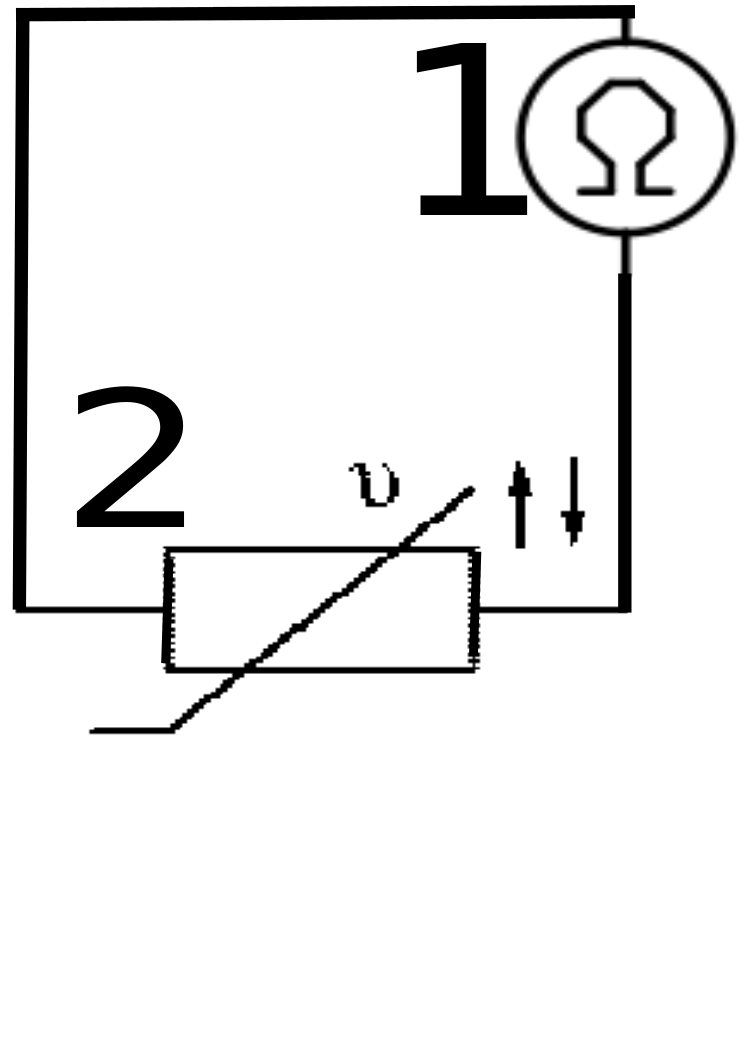
\includegraphics[ scale = 0.1]{Auf_2_2.png}
  	\caption[Schaltskizze zur Messung der Temperatur mit einem NTC]{Schaltskizze zur Messung der Temperatur mit einem NTC\footnotemark}
  \label{fig:auf_2_2}
\end{figure}
\footnotetext{Abbildungsteile entnommen von http://www.atlas.uni-wuppertal.de/$\sim$kind/ep6\_14.pdf am 01.12.2014}

\subsubsection*{Versuchsdurchführung}
%erklären, !was! wir machen, !warum! wir das machen und mit welchem ziel
%(wichtig) präzize erklären, wie bei dem versuch vorgegangen und was gemacht wurde


Der PTC wird an das DMM angeschlossen und der Widerstand bei Raumtemperatur und bei Handtemperatur gemessen.

\subsubsection*{Messergebnisse}
%die messwerte in !übersichtlichen! tabellen angegeben
%zu viele kleine tabellen in große tabellen überführen!
%zu große tabellen mit dem [scale]-befehl scalieren oder (falls zu lang) in zwei kleinere tabellen aufteilen
%(wichtig) vor !jeder! tabelle sagen, was gemessen wurde und wie die fehler gewählt wurden und ausreichend !erklären!, !warum! wir unsere fehler grade so gewählt haben

Die Fehler des Widerstandes wurde mit dem angegebenen Fehler und der Ableseungenauigkeit bestimmt und beträgt 6$\Omega$. Der Fehler der Temperatur wurde über die Ableseungenauigkeit bestimmt und beträgt 0,1C.

\begin{table}[H]
\begin{center}
\begin{tabular}{|r|r|}
\hline
\multicolumn{1}{|l|}{Temperatur/C} & \multicolumn{1}{l|}{Widerstand/$\Omega$} \\ \hline
25,1 & 10330 \\ \hline
35,5 & 8050 \\ \hline
\end{tabular}
\end{center}
\caption{Widerstand in Abhängigkeit der Temperatur}
\label{tab:2_2}
\end{table}


\subsubsection*{Auswertung}
%zuerst !alle! errechneten werte entweder in ganzen sätzen aufzählen, oder in tabellen (übersichtlicher) dargestellen, sowie auf die verwendeten formeln verweisen (die referenzierung der formel kann in der überschrift stehen)
%kurz erwähnen (vor der tabelle), warum wir das ganze ausrechnen bzw. was wir dort ausrechnen
%danach histogramme und plots erstellen, wobei wenn möglich funktionen durch die plots gelegt werden (zur not können auch splines benutzt werden, was aber angegeben werden muss)
%bei fits immer die funktion und das reduzierte chiquadrat mit angegeben, wobei auf verständlichkeit beim entziffern der zehnerpotenzen geachtet werden muss z.b. f(x)=(wert+-fehler)\cdot10^{irgendeine zahl}\cdot x + (wert+-fehler)\cdot10^{irgendeine zahl}
%bei jedem fit erklären, nach welchem zusammenhang gefittet wurde und warum!
%bei plots darauf achten, dass die achsenbeschriftung (auch die tics) die richtige größe haben und die legende im plot nicht die messwerte verdeckt
%kurz die aufgabenstellung abhandeln
%2-----------------------------------------------2
\subsubsection*{Diskussion}
%(immer) die gemessenen werte und die bestimmten werte über die messfehler mit literaturwerten oder untereinander vergleichen
%in welchem fehlerintervall des messwertes liegt der literaturwert oder der vergleichswert?
%wie ist der relative anteil des fehlers am messwert und damit die qualität unserer messung?
%in einem satz erklären, wie gut unser fehler und damit unsere messung ist
%kurz erläutern, wie systematische fehler unsere messung beeinflusst haben könnten
%(wichtig) zum schluss ansprechen, in wie weit die ergebnisse mit der theoretischen vorhersage übereinstimmen
%--------------------------------------------------------------------------------------------
%falls tabellen mit den messwerten zu lang werden, kann die section mit den messwerten auch hinter der diskussion angefügt bzw. eine section mit dem anhang eingefügt werden.
%1-----------------------------------------------1












\subsection{Thermoelemente}
%kurz das ziel dieses versuchsteiles ansprechen, damit keine zwei überschriften direkt übereinander stehen!
%bei schwierigeren versuchen kann auch der theoretische hintergrund erläutert werden. (mit formeln, herleitungen und erklärungen)

Thermoelemente bestehen aus einem Verbund von zwei verschiedenen Metallen. Sie können sehr große Temperaturbereiche abdecken, z.B. -90$^\circ$C bis 1370$^\circ$C.

\subsubsection*{Verwendete Geräte}
%(immer) eine skizze oder ein foto einfügen, die geräte/materialien !nummerieren! und z.b. eine legende dazu schreiben, besser wäre es das ganze in einem Fließtext gut zu beschreiben.
%falls am anfang des versuches nicht klar ist, was alles verwendet wird, wenn möglich erst am ende ein großes foto von den verwendeten materialien machen!\\

Es werden ein Thermoelement und DVM verwendet.


\subsubsection*{Versuchsaufbau}
%skizze zum versuchsaufbau (oder foto) einfügen,   es muss erklärt werden wie das ganze funktioniert und welche speziellen einstellungen verwendet wurden (z.b. welche knöpfe an den geräten für die messung verdreht wurden)

1 ist das Thermoelement und 2 Das DVM.

\begin{figure}[H] 
  \centering
    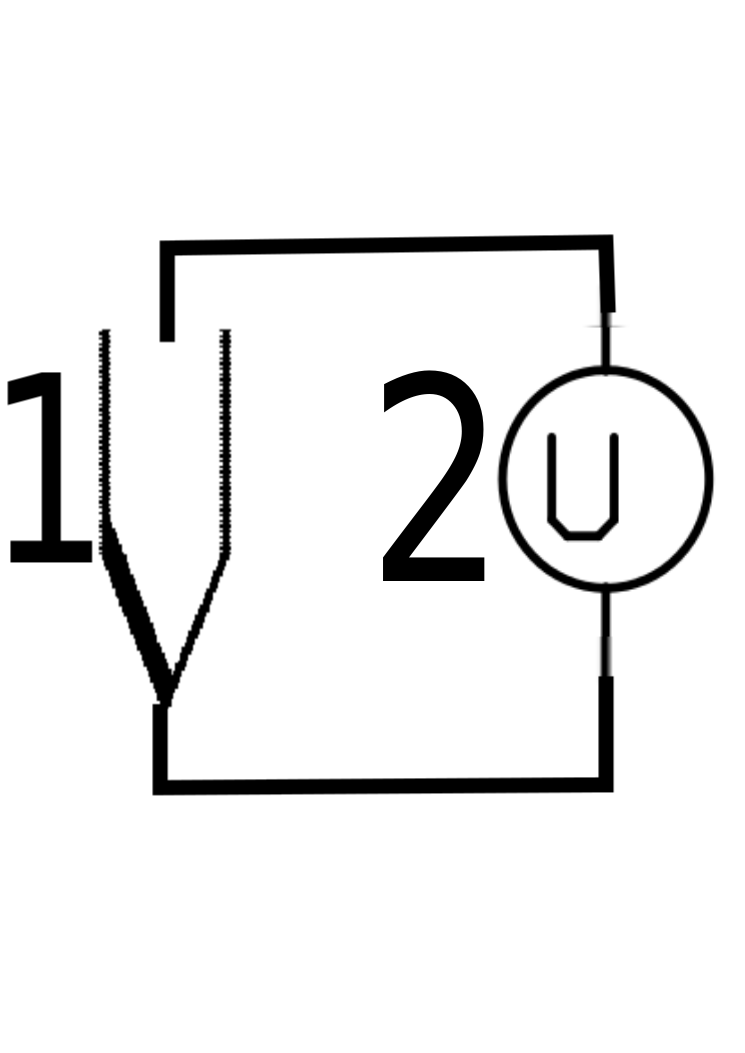
\includegraphics[ scale = 0.1]{2_3.png}
  	\caption[Schaltskizze zum betreiben des Thermoelements]{Schaltskizze zum betreiben des Thermoelements}
  \label{fig:2_3}
\end{figure}

\subsubsection*{Versuchsdurchführung}
%erklären, !was! wir machen, !warum! wir das machen und mit welchem ziel
%(wichtig) präzize erklären, wie bei dem versuch vorgegangen und was gemacht wurde

Das Thermoelement wird an das DVM angeschlossen und die Spannung gemessen.

\subsubsection*{Messergebnisse}
%die messwerte in !übersichtlichen! tabellen angegeben
%zu viele kleine tabellen in große tabellen überführen!
%zu große tabellen mit dem [scale]-befehl scalieren oder (falls zu lang) in zwei kleinere tabellen aufteilen
%(wichtig) vor !jeder! tabelle sagen, was gemessen wurde und wie die fehler gewählt wurden und ausreichend !erklären!, !warum! wir unsere fehler grade so gewählt haben

Die Fehler des Widerstandes wurde mit dem angegebenen Fehler und der Ableseungenauigkeit bestimmt und beträgt0,06mV. Der Fehler der Temperatur wurde über die Ableseungenauigkeit bestimmt und beträgt 0,1C.


\begin{table}[H]
\begin{center}
\begin{tabular}{|r|r|}
\hline
\multicolumn{1}{|l|}{Temperatur/C} & \multicolumn{1}{l|}{Spannung/mV} \\ \hline
33,3 & 6 \\ \hline
\end{tabular}
\end{center}
\caption{Spannung in Abhängigkeit der Temperatur}
\label{tab:2_3}
\end{table}


\subsubsection*{Auswertung}
%zuerst !alle! errechneten werte entweder in ganzen sätzen aufzählen, oder in tabellen (übersichtlicher) dargestellen, sowie auf die verwendeten formeln verweisen (die referenzierung der formel kann in der überschrift stehen)
%kurz erwähnen (vor der tabelle), warum wir das ganze ausrechnen bzw. was wir dort ausrechnen
%danach histogramme und plots erstellen, wobei wenn möglich funktionen durch die plots gelegt werden (zur not können auch splines benutzt werden, was aber angegeben werden muss)
%bei fits immer die funktion und das reduzierte chiquadrat mit angegeben, wobei auf verständlichkeit beim entziffern der zehnerpotenzen geachtet werden muss z.b. f(x)=(wert+-fehler)\cdot10^{irgendeine zahl}\cdot x + (wert+-fehler)\cdot10^{irgendeine zahl}
%bei jedem fit erklären, nach welchem zusammenhang gefittet wurde und warum!
%bei plots darauf achten, dass die achsenbeschriftung (auch die tics) die richtige größe haben und die legende im plot nicht die messwerte verdeckt
%kurz die aufgabenstellung abhandeln
%2-----------------------------------------------2

Es wurde eine Spannung von 6,0$\pm$0,6 mV bei Erwärmung mit der Hand (33,3C) gemessen.

\subsubsection*{Diskussion}
%(immer) die gemessenen werte und die bestimmten werte über die messfehler mit literaturwerten oder untereinander vergleichen
%in welchem fehlerintervall des messwertes liegt der literaturwert oder der vergleichswert?
%wie ist der relative anteil des fehlers am messwert und damit die qualität unserer messung?
%in einem satz erklären, wie gut unser fehler und damit unsere messung ist
%kurz erläutern, wie systematische fehler unsere messung beeinflusst haben könnten
%(wichtig) zum schluss ansprechen, in wie weit die ergebnisse mit der theoretischen vorhersage übereinstimmen
%--------------------------------------------------------------------------------------------
%falls tabellen mit den messwerten zu lang werden, kann die section mit den messwerten auch hinter der diskussion angefügt bzw. eine section mit dem anhang eingefügt werden.
%1-----------------------------------------------1

PTCs lassen sich gut für Messungen mit einer kleinen Temperaturbandbreite, wo man die Temperatur leicht abgelesen können soll. NTCs können gut eingesetzt werden, wenn bei zu geringer Temperatur kein Strom mehr fließen soll. Thermoelemente können gut eingesetzt werden, wenn ein großer Temperaturbereich abgedeckt werden soll. 









\section{Induktion}
%kurz das ziel dieses versuchsteiles ansprechen, damit keine zwei überschriften direkt übereinander stehen!
%bei schwierigeren versuchen kann auch der theoretische hintergrund erläutert werden. (mit formeln, herleitungen und erklärungen)

Mittels Induktion kann ein Magnetfeld vermessen werden. In diesem Versuchsteil wird mit Draht eine Spule gebaut und mit ihr durch messen der Induktionsspannung das Magnetfeld gemessen.

\subsection*{Verwendete Geräte}
%(immer) eine skizze oder ein foto einfügen, die geräte/materialien !nummerieren! und z.b. eine legende dazu schreiben, besser wäre es das ganze in einem Fließtext gut zu beschreiben.
%falls am anfang des versuches nicht klar ist, was alles verwendet wird, wenn möglich erst am ende ein großes foto von den verwendeten materialien machen!\\

Es werden ein Blatt Papier, Kupferdraht, ein Oszilloskop und ein Adapter, mit dem der Draht an das Oszilloskop angeschlossen werden kann.


\subsection*{Versuchsaufbau}
%skizze zum versuchsaufbau (oder foto) einfügen,   es muss erklärt werden wie das ganze funktioniert und welche speziellen einstellungen verwendet wurden (z.b. welche knöpfe an den geräten für die messung verdreht wurden)

Mit dem Kupferdraht wird eine Spule mit wenigen Windungen gebaut, dann wird ein Blatt Papier genommen und zu einem Zylinder mit ca. 2cm Durchmesser gedreht. Um den Papierzylinder werde 100 Windungen mit dem Kupferdraht aufgedreht und an das Oszilloskop angeschlossen.


\subsection*{Versuchsdurchführung}
%erklären, !was! wir machen, !warum! wir das machen und mit welchem ziel
%(wichtig) präzize erklären, wie bei dem versuch vorgegangen und was gemacht wurde

Es wird veränderliches Magnetfeld erzeugt, indem man eine Dauermagnet durch die Spule fallen lässt. Die Induktionsspannung wird auf dem Oszilloskop aufgenommen.


\subsection*{Auswertung}
%zuerst !alle! errechneten werte entweder in ganzen sätzen aufzählen, oder in tabellen (übersichtlicher) dargestellen, sowie auf die verwendeten formeln verweisen (die referenzierung der formel kann in der überschrift stehen)
%kurz erwähnen (vor der tabelle), warum wir das ganze ausrechnen bzw. was wir dort ausrechnen
%danach histogramme und plots erstellen, wobei wenn möglich funktionen durch die plots gelegt werden (zur not können auch splines benutzt werden, was aber angegeben werden muss)
%bei fits immer die funktion und das reduzierte chiquadrat mit angegeben, wobei auf verständlichkeit beim entziffern der zehnerpotenzen geachtet werden muss z.b. f(x)=(wert+-fehler)\cdot10^{irgendeine zahl}\cdot x + (wert+-fehler)\cdot10^{irgendeine zahl}
%bei jedem fit erklären, nach welchem zusammenhang gefittet wurde und warum!
%bei plots darauf achten, dass die achsenbeschriftung (auch die tics) die richtige größe haben und die legende im plot nicht die messwerte verdeckt
%kurz die aufgabenstellung abhandeln
%2-----------------------------------------------2

Lässt man den Permanentmagneten durch die Spule fallen, ergibt sich der Verlauf aus Abbildung \ref{fig:3}. Das der zweite Peak größer ist als der erste, kommt daher, dass sich der Magnet beim verlassen der Spule schneller bewegt als beim eintreten.

\begin{figure}[H] 
  \centering
    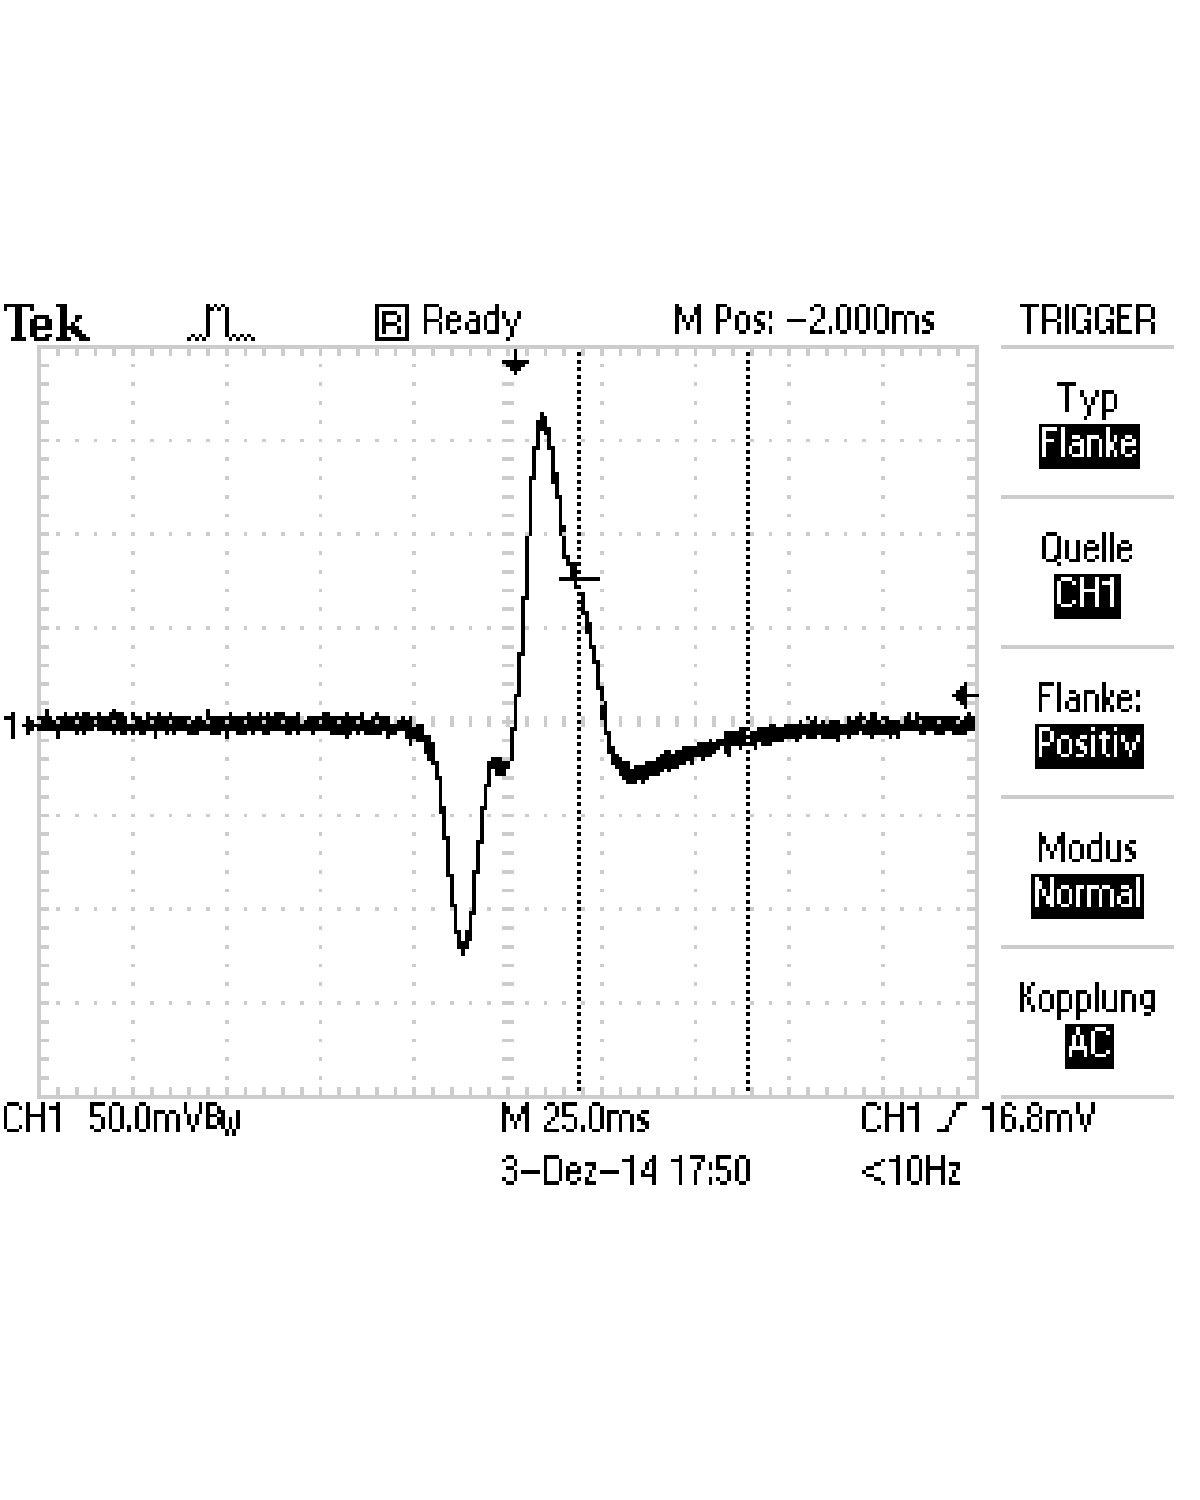
\includegraphics[ scale = 0.7]{3.pdf}
  	\caption[Aufnahme Induktionsspannung]{Aufnahme Induktionsspannung}
  \label{fig:3}
\end{figure}


\subsection*{Diskussion}
%(immer) die gemessenen werte und die bestimmten werte über die messfehler mit literaturwerten oder untereinander vergleichen
%in welchem fehlerintervall des messwertes liegt der literaturwert oder der vergleichswert?
%wie ist der relative anteil des fehlers am messwert und damit die qualität unserer messung?
%in einem satz erklären, wie gut unser fehler und damit unsere messung ist
%kurz erläutern, wie systematische fehler unsere messung beeinflusst haben könnten
%(wichtig) zum schluss ansprechen, in wie weit die ergebnisse mit der theoretischen vorhersage übereinstimmen
%--------------------------------------------------------------------------------------------
%falls tabellen mit den messwerten zu lang werden, kann die section mit den messwerten auch hinter der diskussion angefügt bzw. eine section mit dem anhang eingefügt werden.
%1-----------------------------------------------1

Wie erwartet konnte das zeitlich ändernde Magnetfeld mit der Spule gemessen werden.




\section{Kraft}

Kraft kann über zwei verschiedene Wege in ein elektrisches Signal umgewandelt werden. Dies kann einmal über einen Dehnungsstreifen oder über den piezoelektrischen Effekt realisiert werden. In diesem Versuchsteil werden beide Methoden untersucht.

\subsection{Elementare Dehnungsmessstreifen}
%kurz das ziel dieses versuchsteiles ansprechen, damit keine zwei überschriften direkt übereinander stehen!
%bei schwierigeren versuchen kann auch der theoretische hintergrund erläutert werden. (mit formeln, herleitungen und erklärungen)

Der Dehnungsstreifen besteht aus einer dünnen Schicht Widerstandsdraht, welcher in Kunststoff eingebunden ist. Durch dehnen bzw. stauchen steigt bzw. sinkt der Widerstand, da der Widerstandsdraht länger/kürzer gemacht wird und die Dicke ab- bzw. zunimmt.

\subsubsection*{Verwendete Geräte}
%(immer) eine skizze oder ein foto einfügen, die geräte/materialien !nummerieren! und z.b. eine legende dazu schreiben, besser wäre es das ganze in einem Fließtext gut zu beschreiben.
%falls am anfang des versuches nicht klar ist, was alles verwendet wird, wenn möglich erst am ende ein großes foto von den verwendeten materialien machen!\\

Es werden ein Dehnungsstreifen und dein DMM verwendet.


\subsubsection*{Versuchsaufbau}
%skizze zum versuchsaufbau (oder foto) einfügen,   es muss erklärt werden wie das ganze funktioniert und welche speziellen einstellungen verwendet wurden (z.b. welche knöpfe an den geräten für die messung verdreht wurden)



\begin{figure}[H] 
  \centering
    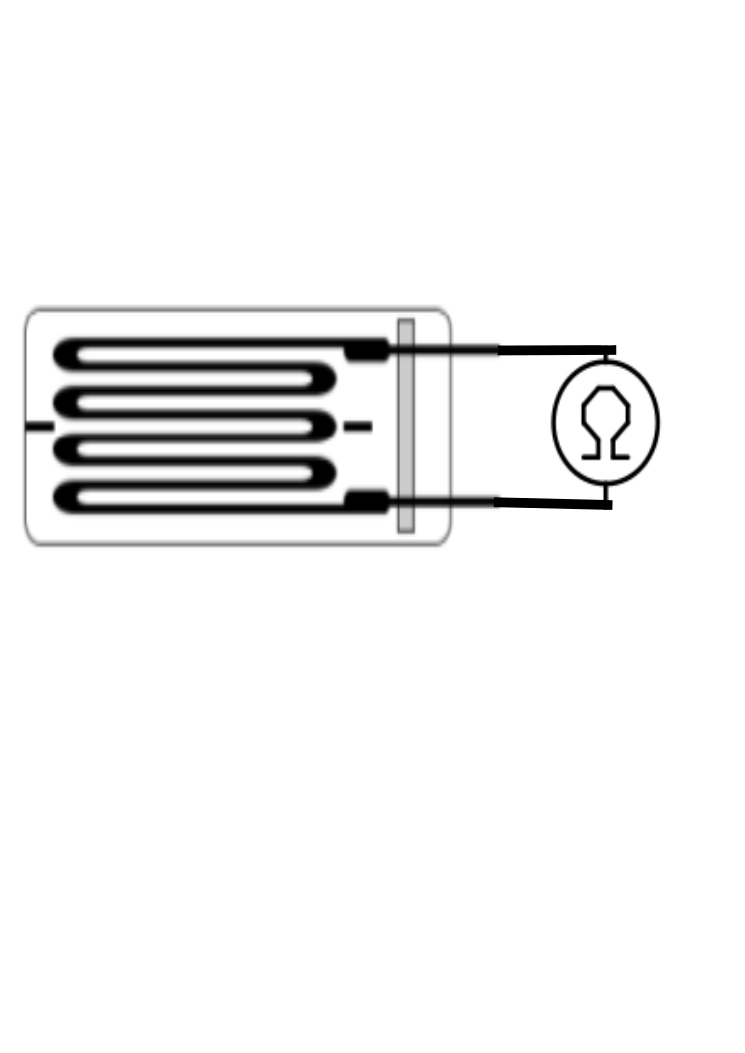
\includegraphics[ scale = 0.1]{auf_4_1.png}
  	\caption[Schaltskizze zur Messung der Kraft mit einem Dehnungsstreifen]{Schaltskizze zur Messung der Kraft mit einem Dehnungsstreifen}
  \label{fig:auf_4_1}
\end{figure}

\subsubsection*{Versuchsdurchführung}
%erklären, !was! wir machen, !warum! wir das machen und mit welchem ziel
%(wichtig) präzize erklären, wie bei dem versuch vorgegangen und was gemacht wurde

Es wird der Versuch nach Abbildung \ref{fig:auf_4_1} aufgebaut und danach der Widerstand bei Stauchung, Ruhelage und Dehnung mit dem DMM gemessen.

\subsubsection*{Messergebnisse}
%die messwerte in !übersichtlichen! tabellen angegeben
%zu viele kleine tabellen in große tabellen überführen!
%zu große tabellen mit dem [scale]-befehl scalieren oder (falls zu lang) in zwei kleinere tabellen aufteilen
%(wichtig) vor !jeder! tabelle sagen, was gemessen wurde und wie die fehler gewählt wurden und ausreichend !erklären!, !warum! wir unsere fehler grade so gewählt haben

Der Fehler des Widerstandes wurde mit dem angegebenem Fehler und dem Ablesefehler bestimmt und beträgt 0,6$\Omega$.

\begin{table}[H]
\begin{center}
\begin{tabular}{|l|r|}
\hline
Zustand & \multicolumn{1}{l|}{Widerstand/$\Omega$} \\ \hline
Stauchung & 119,8 \\ \hline
Ruhelage & 120 \\ \hline
Dehnung & 120,1 \\ \hline
\end{tabular}
\end{center}
\caption{Widerstand in Abhängigkeit des Zustandes, des Dehnungsstreifens}
\label{tab:4_1}
\end{table}


\subsubsection*{Auswertung}
%zuerst !alle! errechneten werte entweder in ganzen sätzen aufzählen, oder in tabellen (übersichtlicher) dargestellen, sowie auf die verwendeten formeln verweisen (die referenzierung der formel kann in der überschrift stehen)
%kurz erwähnen (vor der tabelle), warum wir das ganze ausrechnen bzw. was wir dort ausrechnen
%danach histogramme und plots erstellen, wobei wenn möglich funktionen durch die plots gelegt werden (zur not können auch splines benutzt werden, was aber angegeben werden muss)
%bei fits immer die funktion und das reduzierte chiquadrat mit angegeben, wobei auf verständlichkeit beim entziffern der zehnerpotenzen geachtet werden muss z.b. f(x)=(wert+-fehler)\cdot10^{irgendeine zahl}\cdot x + (wert+-fehler)\cdot10^{irgendeine zahl}
%bei jedem fit erklären, nach welchem zusammenhang gefittet wurde und warum!
%bei plots darauf achten, dass die achsenbeschriftung (auch die tics) die richtige größe haben und die legende im plot nicht die messwerte verdeckt
%kurz die aufgabenstellung abhandeln
%2-----------------------------------------------2

Wie an den Werten in Tabelle \ref{tab:4_1} zu sehen ist die Änderung bei Stauchung und Streckung sehr gering.

\subsubsection*{Diskussion}
%(immer) die gemessenen werte und die bestimmten werte über die messfehler mit literaturwerten oder untereinander vergleichen
%in welchem fehlerintervall des messwertes liegt der literaturwert oder der vergleichswert?
%wie ist der relative anteil des fehlers am messwert und damit die qualität unserer messung?
%in einem satz erklären, wie gut unser fehler und damit unsere messung ist
%kurz erläutern, wie systematische fehler unsere messung beeinflusst haben könnten
%(wichtig) zum schluss ansprechen, in wie weit die ergebnisse mit der theoretischen vorhersage übereinstimmen
%--------------------------------------------------------------------------------------------
%falls tabellen mit den messwerten zu lang werden, kann die section mit den messwerten auch hinter der diskussion angefügt bzw. eine section mit dem anhang eingefügt werden.
%1-----------------------------------------------1

Wie erwartet sind die Widerstandsänderungen sehr gering.







\subsection{Dehnungsmessstreifen in Wheatstonscher Messbrücke, Wägezelle}
%kurz das ziel dieses versuchsteiles ansprechen, damit keine zwei überschriften direkt übereinander stehen!
%bei schwierigeren versuchen kann auch der theoretische hintergrund erläutert werden. (mit formeln, herleitungen und erklärungen)

Bei der Wägelzelle wir über eine Wheatstonsche Brücke ein exakteres Messen der Kraft ermöglicht.

\subsubsection*{Verwendete Geräte}
%(immer) eine skizze oder ein foto einfügen, die geräte/materialien !nummerieren! und z.b. eine legende dazu schreiben, besser wäre es das ganze in einem Fließtext gut zu beschreiben.
%falls am anfang des versuches nicht klar ist, was alles verwendet wird, wenn möglich erst am ende ein großes foto von den verwendeten materialien machen!\\

Es werden eine Wägezelle, ein DMM, ein Netzgerät und ein variables Gewicht verwendet.


\subsubsection*{Versuchsaufbau}
%skizze zum versuchsaufbau (oder foto) einfügen,   es muss erklärt werden wie das ganze funktioniert und welche speziellen einstellungen verwendet wurden (z.b. welche knöpfe an den geräten für die messung verdreht wurden)

1 ist das variable Gewicht und 2 die Wägelzelle. An das Kabel werden noch die 10V Spannungsversorgung(roter und schwarzer Stecker) und das DMM (grüne Stecker) angeschlossen.

\begin{figure}[H] 
  \centering
    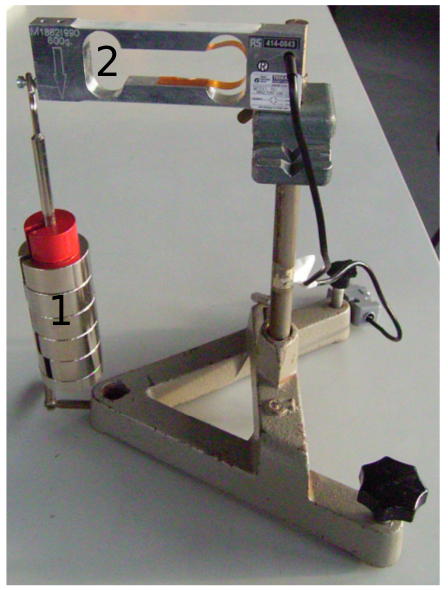
\includegraphics[ scale = 0.3]{auf_4_2.png}
  	\caption[Aufbau zur Kraftmessung mit der Wägezelle]{Aufbau zur Kraftmessung mit der Wägezelle\footnotemark}
  \label{fig:auf_4_2}
\end{figure}
\footnotetext{Abbildung entnommen von http://www.atlas.uni-wuppertal.de/$\sim$kind/ep6\_14.pdf Seite 9 am 01.12.2014}

\subsubsection*{Versuchsdurchführung}
%erklären, !was! wir machen, !warum! wir das machen und mit welchem ziel
%(wichtig) präzize erklären, wie bei dem versuch vorgegangen und was gemacht wurde

Es wird der Versuch nach Abbildung \ref{fig:auf_4_2} und der Beschreibung aufgebaut. Dann werden Gewicht von 0g bis 600g an die Wägezelle angehängt und die Spannung gemessen. Zudem wird im Bereich von 100g bis 150g noch einmal in 10g Schritten gemessen, um die Exaktheit der Wägezelle zu verdeutlichen.

\subsubsection*{Messergebnisse}
%die messwerte in !übersichtlichen! tabellen angegeben
%zu viele kleine tabellen in große tabellen überführen!
%zu große tabellen mit dem [scale]-befehl scalieren oder (falls zu lang) in zwei kleinere tabellen aufteilen
%(wichtig) vor !jeder! tabelle sagen, was gemessen wurde und wie die fehler gewählt wurden und ausreichend !erklären!, !warum! wir unsere fehler grade so gewählt haben

Der Fehler für die Spannung wurde mit der Ableseungenauigkeit und dem angegebenem Fehler bestimmt. Der Fehler beträgt 0,06mV. 

\begin{table}[H]
\begin{center}
\begin{tabular}{|r|r|r|}
\hline
\multicolumn{1}{|l|}{Gewicht/g} & \multicolumn{1}{l|}{Spannung/mV} & \multicolumn{1}{l|}{Spannung pro Volt} \\ \hline
0 & -0,1 & -0,01 \\ \hline
50 & 0,6 & 0,06 \\ \hline
100 & 1,3 & 0,13 \\ \hline
110 & 1,4 & 0,14 \\ \hline
120 & 1,6 & 0,16 \\ \hline
130 & 1,7 & 0,17 \\ \hline
140 & 1,9 & 0,19 \\ \hline
150 & 2 & 0,2 \\ \hline
200 & 2,7 & 0,27 \\ \hline
250 & 3,5 & 0,35 \\ \hline
300 & 4,2 & 0,42 \\ \hline
350 & 4,9 & 0,49 \\ \hline
400 & 5,6 & 0,56 \\ \hline
450 & 6,4 & 0,64 \\ \hline
500 & 7,1 & 0,71 \\ \hline
550 & 7,8 & 0,78 \\ \hline
600 & 8,5 & 0,85 \\ \hline
\end{tabular}
\end{center}
\caption{Spannung in Abhängigkeit des Gewichtes und die Spannung pro Volt in Abhängigkeit des Gewichtes}
\label{tab:4_2}
\end{table}


\subsubsection*{Auswertung}
%zuerst !alle! errechneten werte entweder in ganzen sätzen aufzählen, oder in tabellen (übersichtlicher) dargestellen, sowie auf die verwendeten formeln verweisen (die referenzierung der formel kann in der überschrift stehen)
%kurz erwähnen (vor der tabelle), warum wir das ganze ausrechnen bzw. was wir dort ausrechnen
%danach histogramme und plots erstellen, wobei wenn möglich funktionen durch die plots gelegt werden (zur not können auch splines benutzt werden, was aber angegeben werden muss)
%bei fits immer die funktion und das reduzierte chiquadrat mit angegeben, wobei auf verständlichkeit beim entziffern der zehnerpotenzen geachtet werden muss z.b. f(x)=(wert+-fehler)\cdot10^{irgendeine zahl}\cdot x + (wert+-fehler)\cdot10^{irgendeine zahl}
%bei jedem fit erklären, nach welchem zusammenhang gefittet wurde und warum!
%bei plots darauf achten, dass die achsenbeschriftung (auch die tics) die richtige größe haben und die legende im plot nicht die messwerte verdeckt
%kurz die aufgabenstellung abhandeln
%2-----------------------------------------------2

Da ein linearer Zusammenhang zwischen dem Gewicht und der Spannung vermutet wird, werden die Messdaten aus Tabelle \ref{tab:4_2} mit der Funktion f(x)=m$\cdot$x+b gefittet. Die graphische Auswertung der Messwerte ist in Abbildung \ref{fig:4_2} dargestellt. Durch den Fit ergibt sich f(x)=0.01443($\pm$0,0004)$\cdot$x-0.142716($\pm$0.01), das reduzierte Chi-Quadrat ergibt sich mit 0,26 was für eine sehr gute Übereinstimmung der Messwerte mit der Theorie spricht.

\begin{figure}[H] 
  \centering
    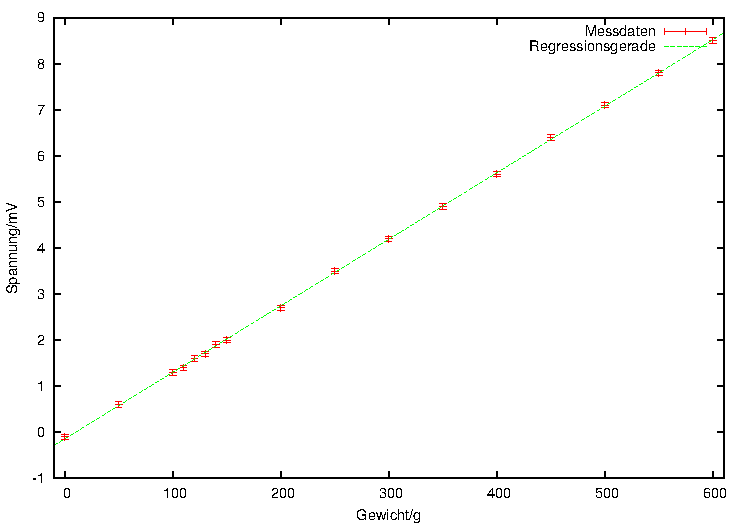
\includegraphics[ scale = 0.7]{4_2.pdf}
  	\caption[Schaltskizze zur Messung der Kraft mit einem Dehnungsstreifen]{Schaltskizze zur Messung der Kraft mit einem Dehnungsstreifen}
  \label{fig:4_2}
\end{figure}

Die Kalibrationswerte für 0g und 600g wurden mit -0,01 mv/V und 0,85 mV/V bestimmt.

\subsubsection*{Diskussion}
%(immer) die gemessenen werte und die bestimmten werte über die messfehler mit literaturwerten oder untereinander vergleichen
%in welchem fehlerintervall des messwertes liegt der literaturwert oder der vergleichswert?
%wie ist der relative anteil des fehlers am messwert und damit die qualität unserer messung?
%in einem satz erklären, wie gut unser fehler und damit unsere messung ist
%kurz erläutern, wie systematische fehler unsere messung beeinflusst haben könnten
%(wichtig) zum schluss ansprechen, in wie weit die ergebnisse mit der theoretischen vorhersage übereinstimmen
%--------------------------------------------------------------------------------------------
%falls tabellen mit den messwerten zu lang werden, kann die section mit den messwerten auch hinter der diskussion angefügt bzw. eine section mit dem anhang eingefügt werden.
%1-----------------------------------------------1

Es konnte sehr gut der lineare Zusammenhang zwischen der Kraft und der Spannung gezeigt werden. Als Kalibrationswerte wurden für 0g -0,0094 mV/V und für 600g 0,8569 mv/V in der Praktikumsanleitung angegeben. Die von uns bestimmten Kalibrationswerte liegen bei -0,01 mV/V für 0g und 0,85 mV/V für 600g, was zeigt, dass die Messung sehr erfolgreich war.

\section{Luftdruckschwankungen/Schall}


\subsection{Dynamische Mikrofone}
%kurz das ziel dieses versuchsteiles ansprechen, damit keine zwei überschriften direkt übereinander stehen!
%bei schwierigeren versuchen kann auch der theoretische hintergrund erläutert werden. (mit formeln, herleitungen und erklärungen)
\subsubsection*{Verwendete Geräte}
%(immer) eine skizze oder ein foto einfügen, die geräte/materialien !nummerieren! und z.b. eine legende dazu schreiben, besser wäre es das ganze in einem Fließtext gut zu beschreiben.
%falls am anfang des versuches nicht klar ist, was alles verwendet wird, wenn möglich erst am ende ein großes foto von den verwendeten materialien machen!\\
\subsubsection*{Verwendete Formeln}
%eine legende kann angefertigt werden, die selbstverständlichen buchstaben müssen nicht extra erklärt werden
%mit knappen erklärungen die !verwendeten! formeln, sowie die zugehörige fehlerrechnung einfügen
%2-----------------------------------------------2
%ab hier kann nochmal in einzelne versuchsteile unterteilt werden
\subsubsection*{Versuchsaufbau}
%skizze zum versuchsaufbau (oder foto) einfügen,   es muss erklärt werden wie das ganze funktioniert und welche speziellen einstellungen verwendet wurden (z.b. welche knöpfe an den geräten für die messung verdreht wurden)
\subsubsection*{Versuchsdurchführung}
%erklären, !was! wir machen, !warum! wir das machen und mit welchem ziel
%(wichtig) präzize erklären, wie bei dem versuch vorgegangen und was gemacht wurde

\subsubsection*{Messergebnisse}
%die messwerte in !übersichtlichen! tabellen angegeben
%zu viele kleine tabellen in große tabellen überführen!
%zu große tabellen mit dem [scale]-befehl scalieren oder (falls zu lang) in zwei kleinere tabellen aufteilen
%(wichtig) vor !jeder! tabelle sagen, was gemessen wurde und wie die fehler gewählt wurden und ausreichend !erklären!, !warum! wir unsere fehler grade so gewählt haben
\subsubsection*{Auswertung}
%zuerst !alle! errechneten werte entweder in ganzen sätzen aufzählen, oder in tabellen (übersichtlicher) dargestellen, sowie auf die verwendeten formeln verweisen (die referenzierung der formel kann in der überschrift stehen)
%kurz erwähnen (vor der tabelle), warum wir das ganze ausrechnen bzw. was wir dort ausrechnen
%danach histogramme und plots erstellen, wobei wenn möglich funktionen durch die plots gelegt werden (zur not können auch splines benutzt werden, was aber angegeben werden muss)
%bei fits immer die funktion und das reduzierte chiquadrat mit angegeben, wobei auf verständlichkeit beim entziffern der zehnerpotenzen geachtet werden muss z.b. f(x)=(wert+-fehler)\cdot10^{irgendeine zahl}\cdot x + (wert+-fehler)\cdot10^{irgendeine zahl}
%bei jedem fit erklären, nach welchem zusammenhang gefittet wurde und warum!
%bei plots darauf achten, dass die achsenbeschriftung (auch die tics) die richtige größe haben und die legende im plot nicht die messwerte verdeckt
%kurz die aufgabenstellung abhandeln
%2-----------------------------------------------2
\subsubsection*{Diskussion}
%(immer) die gemessenen werte und die bestimmten werte über die messfehler mit literaturwerten oder untereinander vergleichen
%in welchem fehlerintervall des messwertes liegt der literaturwert oder der vergleichswert?
%wie ist der relative anteil des fehlers am messwert und damit die qualität unserer messung?
%in einem satz erklären, wie gut unser fehler und damit unsere messung ist
%kurz erläutern, wie systematische fehler unsere messung beeinflusst haben könnten
%(wichtig) zum schluss ansprechen, in wie weit die ergebnisse mit der theoretischen vorhersage übereinstimmen
%--------------------------------------------------------------------------------------------
%falls tabellen mit den messwerten zu lang werden, kann die section mit den messwerten auch hinter der diskussion angefügt bzw. eine section mit dem anhang eingefügt werden.
%1-----------------------------------------------1



\subsection{Kondensator- oder Elektretmikrofone}
%kurz das ziel dieses versuchsteiles ansprechen, damit keine zwei überschriften direkt übereinander stehen!
%bei schwierigeren versuchen kann auch der theoretische hintergrund erläutert werden. (mit formeln, herleitungen und erklärungen)
\subsubsection*{Verwendete Geräte}
%(immer) eine skizze oder ein foto einfügen, die geräte/materialien !nummerieren! und z.b. eine legende dazu schreiben, besser wäre es das ganze in einem Fließtext gut zu beschreiben.
%falls am anfang des versuches nicht klar ist, was alles verwendet wird, wenn möglich erst am ende ein großes foto von den verwendeten materialien machen!\\
\subsubsection*{Verwendete Formeln}
%eine legende kann angefertigt werden, die selbstverständlichen buchstaben müssen nicht extra erklärt werden
%mit knappen erklärungen die !verwendeten! formeln, sowie die zugehörige fehlerrechnung einfügen
%2-----------------------------------------------2
%ab hier kann nochmal in einzelne versuchsteile unterteilt werden

Lückenfüller

\subsubsection*{Versuchsaufbau}
%skizze zum versuchsaufbau (oder foto) einfügen,   es muss erklärt werden wie das ganze funktioniert und welche speziellen einstellungen verwendet wurden (z.b. welche knöpfe an den geräten für die messung verdreht wurden)

\begin{figure}[H] 
  \centering
    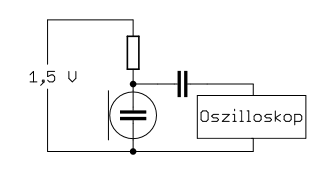
\includegraphics[ scale = 0.7]{Auf_5_2_1.PNG}
  	\caption[Schaltskizze für das Elektretmikrofon]{Schaltskizze für das Elektretmikrofon\footnotemark}
  \label{fig:auf_5_2_1}
\end{figure}
\footnotetext{Abbildung entnommen von http://www.atlas.uni-wuppertal.de/$\sim$kind/ep6\_14.pdf Seite 11 am 01.12.2014}

Lückenfüller

\begin{figure}[H] 
  \centering
    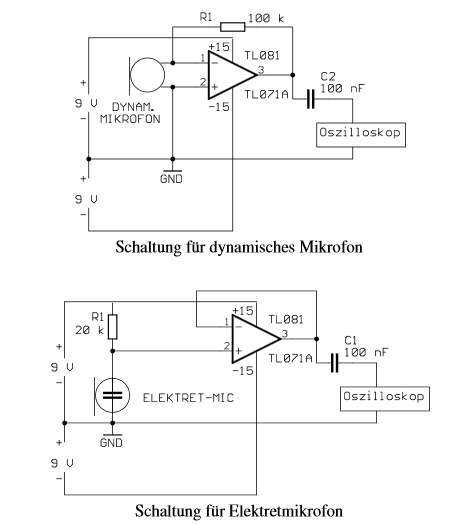
\includegraphics[ scale = 0.7]{Auf_5_2_2.PNG}
  	\caption[Schaltskizze für das Elektretmikrofon und das dynamische Mikrofon mit Operationsverstärker]{Schaltskizze für das Elektretmikrofon und das dynamische Mikrofon mit Operationsverstärker\footnotemark}
  \label{fig:auf_5_2_2}
\end{figure}
\footnotetext{Abbildung entnommen von http://www.atlas.uni-wuppertal.de/$\sim$kind/ep6\_14.pdf Seite 11 am 01.12.2014}

\subsubsection*{Versuchsdurchführung}
%erklären, !was! wir machen, !warum! wir das machen und mit welchem ziel
%(wichtig) präzize erklären, wie bei dem versuch vorgegangen und was gemacht wurde

\subsubsection*{Messergebnisse}
%die messwerte in !übersichtlichen! tabellen angegeben
%zu viele kleine tabellen in große tabellen überführen!
%zu große tabellen mit dem [scale]-befehl scalieren oder (falls zu lang) in zwei kleinere tabellen aufteilen
%(wichtig) vor !jeder! tabelle sagen, was gemessen wurde und wie die fehler gewählt wurden und ausreichend !erklären!, !warum! wir unsere fehler grade so gewählt haben
\subsubsection*{Auswertung}
%zuerst !alle! errechneten werte entweder in ganzen sätzen aufzählen, oder in tabellen (übersichtlicher) dargestellen, sowie auf die verwendeten formeln verweisen (die referenzierung der formel kann in der überschrift stehen)
%kurz erwähnen (vor der tabelle), warum wir das ganze ausrechnen bzw. was wir dort ausrechnen
%danach histogramme und plots erstellen, wobei wenn möglich funktionen durch die plots gelegt werden (zur not können auch splines benutzt werden, was aber angegeben werden muss)
%bei fits immer die funktion und das reduzierte chiquadrat mit angegeben, wobei auf verständlichkeit beim entziffern der zehnerpotenzen geachtet werden muss z.b. f(x)=(wert+-fehler)\cdot10^{irgendeine zahl}\cdot x + (wert+-fehler)\cdot10^{irgendeine zahl}
%bei jedem fit erklären, nach welchem zusammenhang gefittet wurde und warum!
%bei plots darauf achten, dass die achsenbeschriftung (auch die tics) die richtige größe haben und die legende im plot nicht die messwerte verdeckt
%kurz die aufgabenstellung abhandeln
%2-----------------------------------------------2
\subsubsection*{Diskussion}
%(immer) die gemessenen werte und die bestimmten werte über die messfehler mit literaturwerten oder untereinander vergleichen
%in welchem fehlerintervall des messwertes liegt der literaturwert oder der vergleichswert?
%wie ist der relative anteil des fehlers am messwert und damit die qualität unserer messung?
%in einem satz erklären, wie gut unser fehler und damit unsere messung ist
%kurz erläutern, wie systematische fehler unsere messung beeinflusst haben könnten
%(wichtig) zum schluss ansprechen, in wie weit die ergebnisse mit der theoretischen vorhersage übereinstimmen
%--------------------------------------------------------------------------------------------
%falls tabellen mit den messwerten zu lang werden, kann die section mit den messwerten auch hinter der diskussion angefügt bzw. eine section mit dem anhang eingefügt werden.
%1-----------------------------------------------1



\section{Feuchte}
%kurz das ziel dieses versuchsteiles ansprechen, damit keine zwei überschriften direkt übereinander stehen!
%bei schwierigeren versuchen kann auch der theoretische hintergrund erläutert werden. (mit formeln, herleitungen und erklärungen)
\subsection*{Verwendete Geräte}
%(immer) eine skizze oder ein foto einfügen, die geräte/materialien !nummerieren! und z.b. eine legende dazu schreiben, besser wäre es das ganze in einem Fließtext gut zu beschreiben.
%falls am anfang des versuches nicht klar ist, was alles verwendet wird, wenn möglich erst am ende ein großes foto von den verwendeten materialien machen!\\
\subsection*{Verwendete Formeln}
%eine legende kann angefertigt werden, die selbstverständlichen buchstaben müssen nicht extra erklärt werden
%mit knappen erklärungen die !verwendeten! formeln, sowie die zugehörige fehlerrechnung einfügen
%2-----------------------------------------------2
%ab hier kann nochmal in einzelne versuchsteile unterteilt werden
\subsection*{Versuchsaufbau}
%skizze zum versuchsaufbau (oder foto) einfügen,   es muss erklärt werden wie das ganze funktioniert und welche speziellen einstellungen verwendet wurden (z.b. welche knöpfe an den geräten für die messung verdreht wurden)

\begin{figure}[H] 
  \centering
    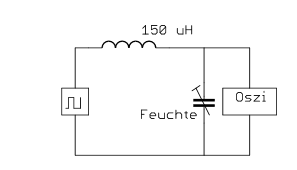
\includegraphics[ scale = 0.7]{Auf_6_1.PNG}
  	\caption[Schaltskizze für die Feuchtigkeitsmessung]{Schaltskizze für die Feuchtigkeitsmessung}
  \label{fig:auf_6}
\end{figure}

\subsection*{Versuchsdurchführung}
%erklären, !was! wir machen, !warum! wir das machen und mit welchem ziel
%(wichtig) präzize erklären, wie bei dem versuch vorgegangen und was gemacht wurde

\subsection*{Messergebnisse}
%die messwerte in !übersichtlichen! tabellen angegeben
%zu viele kleine tabellen in große tabellen überführen!
%zu große tabellen mit dem [scale]-befehl scalieren oder (falls zu lang) in zwei kleinere tabellen aufteilen
%(wichtig) vor !jeder! tabelle sagen, was gemessen wurde und wie die fehler gewählt wurden und ausreichend !erklären!, !warum! wir unsere fehler grade so gewählt haben
\subsection*{Auswertung}
%zuerst !alle! errechneten werte entweder in ganzen sätzen aufzählen, oder in tabellen (übersichtlicher) dargestellen, sowie auf die verwendeten formeln verweisen (die referenzierung der formel kann in der überschrift stehen)
%kurz erwähnen (vor der tabelle), warum wir das ganze ausrechnen bzw. was wir dort ausrechnen
%danach histogramme und plots erstellen, wobei wenn möglich funktionen durch die plots gelegt werden (zur not können auch splines benutzt werden, was aber angegeben werden muss)
%bei fits immer die funktion und das reduzierte chiquadrat mit angegeben, wobei auf verständlichkeit beim entziffern der zehnerpotenzen geachtet werden muss z.b. f(x)=(wert+-fehler)\cdot10^{irgendeine zahl}\cdot x + (wert+-fehler)\cdot10^{irgendeine zahl}
%bei jedem fit erklären, nach welchem zusammenhang gefittet wurde und warum!
%bei plots darauf achten, dass die achsenbeschriftung (auch die tics) die richtige größe haben und die legende im plot nicht die messwerte verdeckt
%kurz die aufgabenstellung abhandeln
%2-----------------------------------------------2
\subsection*{Diskussion}
%(immer) die gemessenen werte und die bestimmten werte über die messfehler mit literaturwerten oder untereinander vergleichen
%in welchem fehlerintervall des messwertes liegt der literaturwert oder der vergleichswert?
%wie ist der relative anteil des fehlers am messwert und damit die qualität unserer messung?
%in einem satz erklären, wie gut unser fehler und damit unsere messung ist
%kurz erläutern, wie systematische fehler unsere messung beeinflusst haben könnten
%(wichtig) zum schluss ansprechen, in wie weit die ergebnisse mit der theoretischen vorhersage übereinstimmen
%--------------------------------------------------------------------------------------------
%falls tabellen mit den messwerten zu lang werden, kann die section mit den messwerten auch hinter der diskussion angefügt bzw. eine section mit dem anhang eingefügt werden.
%1-----------------------------------------------1





\section{Fazit}
%im fazit nochmal alles zusammenfassen und den verlauf der messung abschätzen
%gravierende sytematische probleme bei den messungen nochmal betonen und die wertigkeit unserer ergebnisse einordnen
\end{document}

